\documentclass[a4paper,fleqn]{cas-dc}

\usepackage[spanish,es-tabla,es-nodecimaldot]{babel}
\usepackage[authoryear,round]{natbib}
\bibliographystyle{plainnat}
\newcommand{\autocite}[1]{\citep{#1}}
\newcommand{\parencite}[1]{\citep{#1}}
\usepackage{float}
\usepackage{longtable}
\usepackage{xurl}
% cas-dc ya carga graphicx, amsmath, amssymb, booktabs y hyperref
\graphicspath{{figures/}}
\hypersetup{
    linkcolor=blue,
    filecolor=magenta,
    urlcolor=cyan,
    citecolor=blue
}

% Localización de textos fijos de cas-dc
\ExplSyntaxOn
\cs_set:Npn \__first_footerline: { \small\sffamily TC2035~--~Avance~4 }
\RenewDocumentCommand \printorcid { } { } % evita la línea "ORCID(s):" vacía
\RenewDocumentEnvironment { keywords } { O{ Palabras~clave } }
   {
     \tex_global:D \tex_setbox:D \g_stm_key_box = \vtop \bgroup
     \hsize=.25 \textwidth
     \cs_set:Npn \sep { \par }
     \parindent = 0pt
     I\,N\,F\,O\,R\,M\,A\,C\,I\,Ó\,N \par \skip_vertical:n { -3pt }
     \rule{.25 \textwidth}{.2pt}\par\footnotesize
     \noindent \textit { #1 }:  \par
   }
   { \egroup }
\ExplSyntaxOff

\begin{document}
\let\WriteBookmarks\relax
\def\floatpagepagefraction{1}
\def\textpagefraction{.001}
\shorttitle{Clasificación automática de 104 tipos de flores}
\shortauthors{Eduardo-Luna et al.}

\title [mode = title]{Clasificación automática de 104 tipos de flores con redes neuronales profundas}
\tnotemark[1]
\tnotetext[1]{Situación problema: Red convolutiva, Avance 4. Diseño de Redes Neuronales y Aprendizaje Profundo (TC2035.201). Basado en la competencia \textit{Petals to the Metal -- Flower Classification on TPU} (Kaggle).}

\author[1]{Angel Eduardo-Luna}
\fnmark[1]
\author[1]{Andrea Estefanía De la Peña Contreras}
\fnmark[2]
\author[1]{Jannette Cristina Flores Rodríguez}
\fnmark[3]
\author[1]{Rey Iván de la Fuente Chávez}
\fnmark[4]
\author[1]{Andrés Huerta Robinson}
\fnmark[5]

\affiliation[1]{organization={Escuela de Ingeniería y Ciencias, Tecnológico de Monterrey},
    city={Monterrey},
    state={Nuevo León},
    country={México}}

\fntext[1]{Matrícula: A00842657}
\fntext[2]{Matrícula: A00840973}
\fntext[3]{Matrícula: A01255711}
\fntext[4]{Matrícula: A01709445}
\fntext[5]{Matrícula: A00838626}

\begin{abstract}
Se comparan una red totalmente conectada de referencia, una CNN original de cuatro
convoluciones, una variante con dos convoluciones adicionales y una intervención
de regularización con AdamW y ajuste de tasa. Se utilizan 12,753 imágenes reales
de entrenamiento y 3,712 de validación de 104 categorías de flores, con entrada
$112\times112$. Se incluyen representaciones de las arquitecturas, curvas de
entrenamiento y validación, matrices de confusión y predicciones ilustrativas.
El modelo elegido por F1 macro de validación es CNN + AdamW + LR, con F1 macro 0.5745 y exactitud 64.44\%. 
La red totalmente conectada es una referencia reconstruida, no un checkpoint
histórico identificado del Avance 3. Los resultados corresponden a una sola
semilla y no se presentan como evaluación sobre prueba independiente.
\end{abstract}

\begin{keywords}
Clasificación de imágenes \sep Redes neuronales convolucionales \sep
Regularización \sep F1 macro \sep Flores
\end{keywords}


\maketitle

\section{Resumen y objetivos}
El Entregable 3 desarrolló una CNN para clasificar flores y analizó el conjunto
completo, muestras aleatorias reducidas y datos sintéticos obtenidos mediante
Distribution Matching. Su versión corregida incorporó también evidencia histórica
de hiperparámetros y regularización. El objetivo de esta entrega es ampliar esa
investigación y estudiar
su capacidad de ajuste y generalización. Se comparan una red totalmente conectada
(MLP), una CNN de cuatro convoluciones, una variante de seis convoluciones y
una CNN con AdamW y ajuste de tasa. Se cuantifican F1 macro, exactitud, pérdida,
parámetros y errores por clase. La MLP es una referencia reconstruida con el
pipeline del equipo para contrastar conectividad densa y convolucional: el
Entregable 3 corregido utilizó una CNN, no una MLP.

Para estudiar la regularización se incorpora, en un grupo experimental separado,
el mismo par de corridas históricas ya analizado en el A3 corregido, con y sin dropout, aumento de datos y decaimiento
de pesos. Se presentan tanto sus mejores checkpoints como una comparación en
la misma época registrada. Las curvas y las brechas permiten distinguir mayor
ajuste de train de una mejora efectiva en validación.

\section{Contexto del problema}
Muchas categorías de flores son visualmente parecidas y distinguirlas puede requerir conocimiento especializado. Identificarlas de forma manual es lento cuando se tienen miles de fotografías. Por eso resulta útil contar con modelos que reconozcan la clase de una flor a partir de una imagen.

Este proyecto parte de la competencia "Petals to the Metal", encontrado en Kaggle, cuyo reto es construir un modelo que identifique el tipo de flor en un conjunto de imágenes. La competencia se limita a 104 clases de flores, y consiste en un problema de clasificación multiclase de imágenes en el que el modelo debe tener la capacidad de identificar valores finos como la forma, estructura y color para distinguir entre categorías cercanas. 

Este problema tiene varias dificultades que lo hacen relevante desde un enfoque de redes neuronales. Primeramente, las clases son heterogéneas, ya que algunas de ellas solo tienen un subtipo de flor y otras agrupan muchas subvariedades. Además, las imágenes de las flores no fueron capturadas en el mismo entorno, dando más variedad a las mismas. Por último, el número de imágenes por cada clase tampoco es uniforme, por lo que, considerando la métrica de evaluación, es un punto fuerte a tomar en cuenta que el modelo funcione de manera efectiva tanto para clases con pocos ejemplos como también para aquellas con muchos. 

\section{Descripción del dataset}
\subsection{Datos y particiones}
Se utilizan los TFRecords de la competencia \textit{Petals to the Metal -- Flower
Classification on TPU} \citep{kagglePetalsMetal}, con 104 clases y fotografías
RGB. El conjunto incluye categorías relacionadas con la clasificación fina de
flores, estudiada también en Oxford Flowers \citep{nilsback2008}. Se mantienen
las particiones originales de Kaggle (Tabla~\ref{tab:particiones}).
\begin{table}[htbp]
\centering\small
\caption{Particiones originales utilizadas.}\label{tab:particiones}
\begin{tabular}{lrr}
\toprule Partición & Imágenes & Etiquetas locales \\
\midrule Train & 12,753 & Sí \\ Validación & 3,712 & Sí \\
Test & 7,382 & No \\ Total & 23,847 & \\
\bottomrule
\end{tabular}
\end{table}
Cada registro etiquetado contiene una imagen JPEG y una clase entera de 0 a 103;
test proporciona identificadores para generar predicciones. Se leen los archivos
de origen de $224\times224$, pero la entrada efectiva de todos los modelos
analizados es $112\times112\times3$. No se crea una partición nueva ni se usan
imágenes de validación para actualizar pesos.

\subsection{Desbalance y métricas}
El conteo histórico de train varía entre 18 y 782 imágenes por clase; su promedio
es 122.6. La exactitud global puede favorecer clases numerosas. Por ello el
criterio principal es F1 macro, que pondera por igual las 104 categorías.
Para una clase $c$, con verdaderos positivos $TP_c$, falsos positivos $FP_c$
y falsos negativos $FN_c$:
\begin{equation}
P_c=\frac{TP_c}{TP_c+FP_c},\qquad R_c=\frac{TP_c}{TP_c+FN_c},
\end{equation}
\begin{equation}
F1_c=\frac{2P_cR_c}{P_c+R_c},\qquad F1_{\rm macro}=\frac{1}{104}\sum_{c=0}^{103}F1_c.
\end{equation}
Los denominadores nulos se resuelven asignando cero a la métrica. El soporte es
el número de imágenes reales de esa clase en validación. Se informa también
exactitud y entropía cruzada: esta última penaliza errores de alta confianza
que un cambio de clase predicha no refleja por sí solo.

\section{Algoritmos y aplicaciones}
\subsection{Red totalmente conectada}
La MLP transforma la imagen en un vector $x\in\mathbb{R}^{37,632}$ y aplica
$h=\operatorname{ReLU}(Wx+b)$, dropout y una capa lineal de 104 salidas.
Cada neurona recibe todos los píxeles con pesos independientes por posición.
Esta conectividad permite relaciones globales, pero no incorpora explícitamente
la vecindad espacial ni reutiliza un detector entre regiones. La primera matriz
de 37,632 por 256 domina el costo en parámetros.

\subsection{Convolución, activación y pooling}
Una CNN aplica el mismo kernel a vecindarios de la imagen. De forma esquemática,
un mapa de salida es
\begin{equation}
a_{i,j,k}=\operatorname{ReLU}\!\left(b_k+\sum_{u,v,c}K_{u,v,c,k}x_{i+u,j+v,c}\right).
\end{equation}
La conectividad local conserva relaciones entre píxeles cercanos y los filtros
compartidos reducen parámetros respecto a conectar cada píxel con cada unidad.
La composición de capas permite combinar patrones locales en representaciones
más complejas. El max pooling de $2\times2$ reduce tamaño espacial y aporta
cierta tolerancia a desplazamientos, sin garantizar invariancia completa.
Global average pooling (GAP) promedia cada mapa y evita una gran matriz densa
sobre todas las posiciones. Estas propiedades motivan las CNN para imágenes
\citep{ibmWhatImage}; su ventaja concreta se evalúa empíricamente.

\subsection{Aprendizaje y regularización}
Los modelos producen logits, no una segunda softmax antes de la pérdida. Para
la etiqueta verdadera $c$ se minimiza entropía cruzada dispersa:
\begin{equation}
L=-\log\frac{\exp(z_c)}{\sum_{k=0}^{103}\exp(z_k)}.
\end{equation}
La retropropagación calcula gradientes y Adam actualiza pesos por minilotes.
Dropout desactiva unidades aleatorias durante entrenamiento; los aumentos
presentan variaciones de imágenes reales. AdamW aplica decaimiento de pesos
desacoplado del gradiente de la pérdida. La reducción de tasa en meseta y la
parada temprana controlan el progreso y la selección del checkpoint. Sus efectos
no pueden aislarse cuando varias condiciones cambian simultáneamente.

\subsection{Alternativas y alcance}
KNN, SVM y bosques aleatorios sobre características, así como arquitecturas
preentrenadas, son alternativas posibles; no se presentan como modelos ejecutados
en esta comparación. La aplicación considerada exige clasificar las 104 etiquetas
del dataset, con cautela ante cambios de dominio y clases no conocidas.

\section{Metodología}
\subsection{Arquitecturas entrenadas}
La MLP aplica Flatten, Dense256/ReLU, dropout 0.5 y Dense104; tiene 9,660,776
parámetros. La primera capa aporta 9,634,048 (99.72\%), porque cada uno de los
37,632 valores de entrada se conecta con las 256 unidades, además de sus sesgos.
No contiene convoluciones ni pooling.

La CNN original contiene cuatro Conv $3\times3$, padding \textit{same}, con
32, 64, 128 y 256 filtros, ReLU y max pooling $2\times2$ por bloque. Las salidas
son $56\times56\times32$, $28\times28\times64$, $14\times14\times128$ y
$7\times7\times256$. GAP, Dense256/ReLU, dropout 0.5 y Dense104 completan
480,936 parámetros. La CNN ampliada añade Conv128 después de pool3 y Conv256
después de pool4, ambas $3\times3$/ReLU, sin pool adicional: seis convoluciones
y 1,218,600 parámetros. La variante AdamW/LR conserva la arquitectura original.
\begin{figure*}[htbp]
\centering
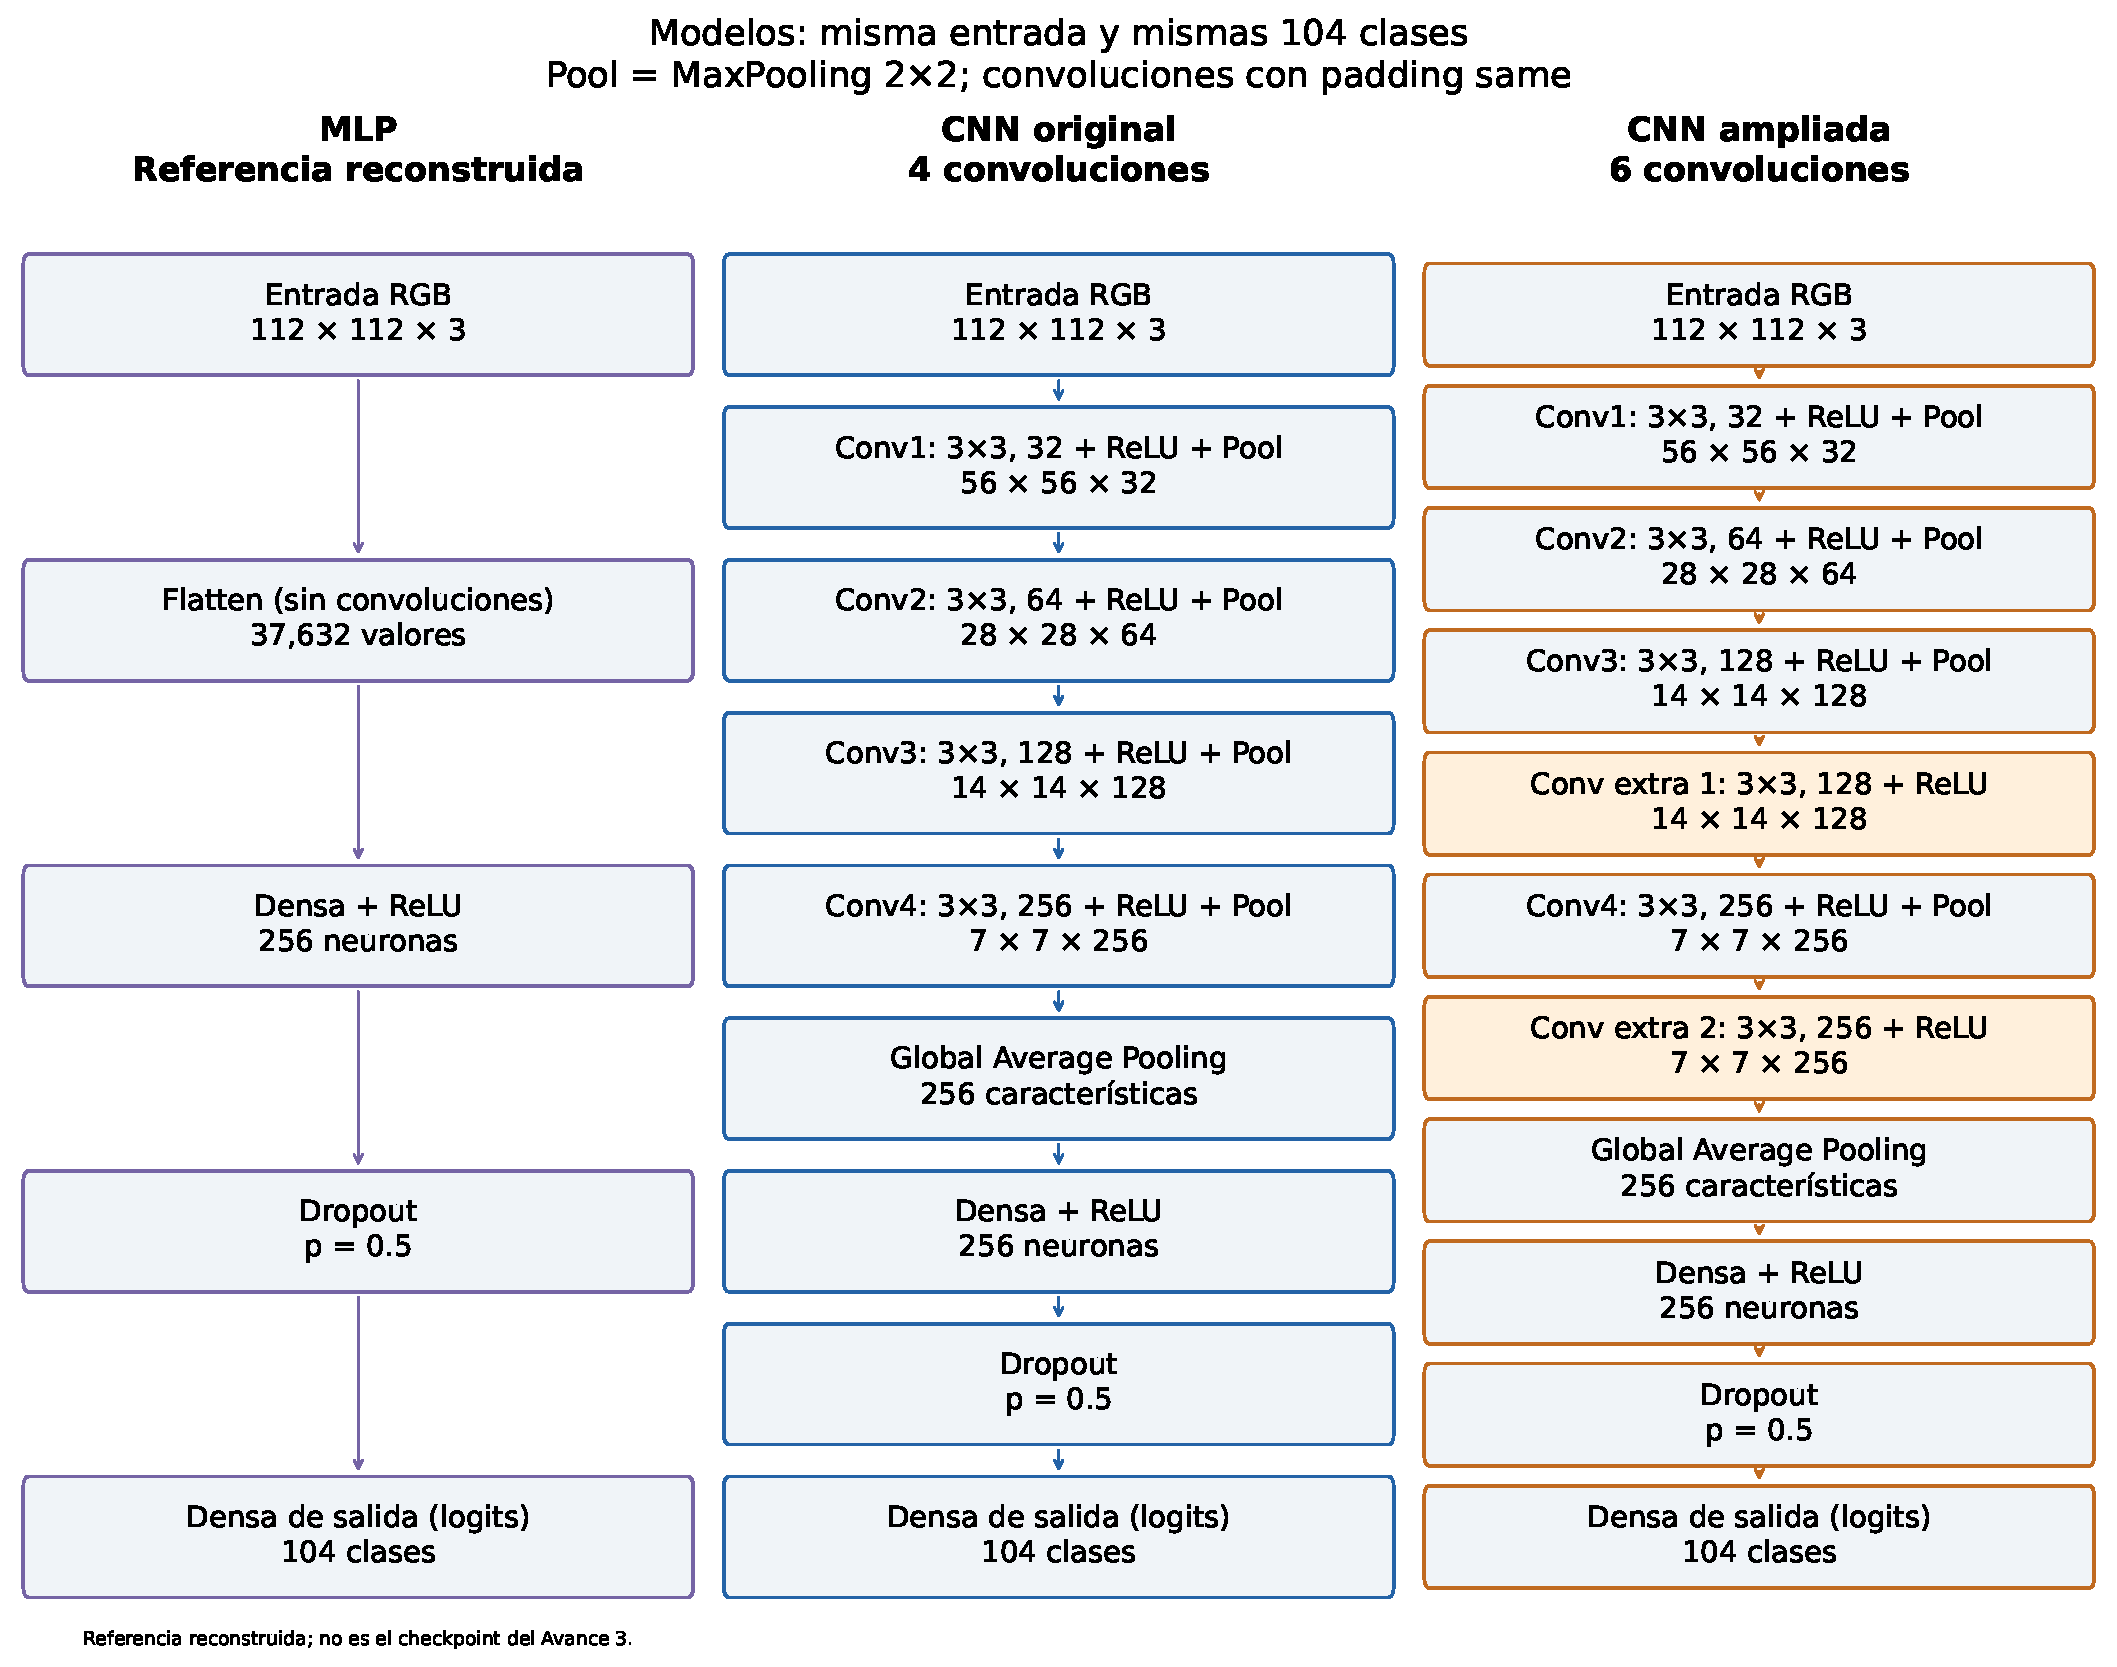
\includegraphics[width=0.93\textwidth,height=0.65\textheight,keepaspectratio]{avance4_2026-10-21/figures/arquitecturas.pdf}
\caption{Arquitecturas históricas A4 con entrada efectiva de 112 por 112. Las capas
adicionales de la CNN ampliada se muestran en naranja.}\label{fig:arquitecturas-av4}
\end{figure*}

\subsection{Preprocesamiento}
El lector decodifica JPEG RGB, convierte a float32, divide por 255 y redimensiona
con interpolación bilineal y antialias a $112\times112$. Train se mezcla y usa
volteo horizontal, rotación de factor 0.05, zoom 0.1 y contraste 0.1; los valores
se recortan a $[0,1]$. La caché precede a los aumentos, que cambian entre épocas.
Validación no usa transformaciones aleatorias. La MLP aplana en orden NHWC,
coherente entre su implementación PyTorch y la exportación Keras.

\subsection{Implementación y procedencia}
Las cuatro corridas A4 se entrenaron históricamente con PyTorch/DirectML en
Radeon RX 6700S y lector TensorFlow; sus checkpoints PT se exportaron a Keras.
Los registros conservan una prueba histórica de paridad sobre un lote. Este
análisis recalcula métricas desde las predicciones guardadas y coteja las pérdidas
con los archivos; no vuelve a ejecutar inferencia sobre imágenes.

El par complementario F procede del reporte final y utiliza TensorFlow/Metal,
según su documentación. No se trata de una repetición DirectML. La destilación
Distribution Matching pertenece a otro experimento del proyecto: no se usaron
sus imágenes sintéticas para entrenar las seis corridas aquí comparadas.

\section{Protocolo experimental y reproducibilidad}
\subsection{Familias y condiciones}
Se distinguen \textbf{A3}: CNN inicial y experimentos aleatorios/DM;
\textbf{A4}: MLP, CNN original, CNN ampliada y CNN AdamW/LR; y
\textbf{F}: hiperparámetros históricos reutilizados en el A3 corregido y
conservados en el reporte final. Las corridas A4 y el par F aquí analizado
declaran seed 0, train completo, la misma validación, entrada 112,
batch 64 y hasta 150 épocas. No se promedian resultados entre familias.

En A4, las CNN original y ampliada usan Adam LR $10^{-3}$ y paciencia de cinco
evaluaciones sin mejora de F1. La MLP usa Adam LR $10^{-4}$, paciencia diez y
mínimo diez épocas, después de un ensayo fallido con $10^{-3}$. La CNN AdamW/LR
usa weight decay 0.01 sin sesgos, reducción por pérdida de validación de factor
0.5, paciencia dos, mínimo $10^{-5}$ y parada temprana de doce evaluaciones.
Todos los A4 usan dropout 0.5 y aumentos: su comparación Adam/AdamW no equivale
a retirar toda la regularización explícita.

En F se compara dropout 0.5, aumentos y AdamW/WD 0.01 frente a dropout 0,
sin aumentos y Adam/WD 0. Ambas conservan LR inicial $10^{-3}$, la misma regla
de reducción de tasa, paciencia doce y tope 150. Sus trayectorias reales de LR
pueden diferir. El checkpoint se selecciona por máximo F1 macro; exactitud y
pérdida se asocian a ese mismo modelo, no a máximos independientes.
El mínimo de pérdida de todo un historial es otra cantidad, obtenida posiblemente
en otra época; no se usa para completar métricas del checkpoint por F1.

\subsection{Medición de la brecha}
En A4, train se mide durante actualizaciones con dropout y aumentos. En F se
registran además las primeras 3,712 imágenes fijas de train, sin aumentos y en
modo inferencia al final de cada época. Solo estas métricas limpias permiten
comparar con validación bajo el mismo modo de evaluación:
\begin{equation}
\Delta F=F1_{\rm train,limpio}-F1_{\rm val}.
\end{equation}
Ese subconjunto no es todo train ni una muestra estratificada. Sus métricas
se recuperan de históricos, sin predicciones individuales de train para repetir
el recálculo. Se comparan mejores checkpoints y, como complemento, la época
34 registrada en ambas corridas F. No se interpolan valores ausentes.

\subsection{Artefactos y límites de ejecución}
Los originales A4 están en
\path{reports/entregable_4/avance4_2026-10-21}; el par F, en
\path{reports/final/experimentos/runs}. Los derivados registran IDs de familia,
rutas y hashes en carpetas de corrección del A4. La tabla completa por clase
se obtiene de predicciones, sin modificar sus fuentes.

El notebook \path{notebooks/equipo_proyecto_avance4.ipynb} del
\href{https://github.com/Lunaaaalj/NeuralNetworksTeamEnvironment}{repositorio del equipo}
separa análisis histórico de entrenamiento. El primer modo usa CSV/JSON sin
frameworks de entrenamiento ni TFRecords; el segundo exige datos y dependencias
y escribe en una salida nueva. En el entorno de revisión faltaron TFRecords y
frameworks, por lo que no se reentrenaron modelos ni se recalcularon pérdidas
sobre imágenes. Una semilla no estima variabilidad; validación también se usa
para seleccionar modelos y no constituye test independiente.

\section{Regularización}

\subsection{Diagnóstico con curvas de entrenamiento y validación}

La Figura~\ref{fig:curvas-av4} compara exactitud y entropía cruzada para cada
modelo. Se muestran todas las épocas ejecutadas y se marca la época seleccionada
por F1 macro. No se confunde la última época con el checkpoint final evaluado.
En una fase de sobreajuste, el modelo sigue reduciendo su error de entrenamiento
sin obtener la misma mejora en validación; en particular, una pérdida de validación
que aumenta revela errores más confiados aunque la exactitud cambie poco.

\begin{itemize}
\item \textbf{MLP de referencia}: la menor pérdida de validación fue 3.339 en la época 76. Al terminar, la pérdida de entrenamiento fue 3.595 y la de validación 3.345; la exactitud de entrenamiento fue 11.78\% y la de validación 15.41\%. Estas curvas deben interpretarse junto con F1 macro; no se concluye sobreajuste solo por una diferencia entre exactitudes.
\item \textbf{CNN original}: la menor pérdida de validación fue 1.520 en la época 53. Al terminar, la pérdida de entrenamiento fue 0.937 y la de validación 1.609; la exactitud de entrenamiento fue 71.17\% y la de validación 62.53\%. La reducción de la pérdida de entrenamiento junto con una pérdida de validación mayor que su mínimo es evidencia de sobreajuste en la fase final.
\item \textbf{CNN + 2 convoluciones}: la menor pérdida de validación fue 1.658 en la época 31. Al terminar, la pérdida de entrenamiento fue 0.564 y la de validación 2.024; la exactitud de entrenamiento fue 82.66\% y la de validación 60.48\%. La reducción de la pérdida de entrenamiento junto con una pérdida de validación mayor que su mínimo es evidencia de sobreajuste en la fase final.
\item \textbf{CNN + AdamW + LR}: la menor pérdida de validación fue 1.494 en la época 52. Al terminar, la pérdida de entrenamiento fue 0.785 y la de validación 1.512; la exactitud de entrenamiento fue 76.16\% y la de validación 64.41\%. Estas curvas deben interpretarse junto con F1 macro; no se concluye sobreajuste solo por una diferencia entre exactitudes.
\end{itemize}

\begin{figure*}[p]
\centering
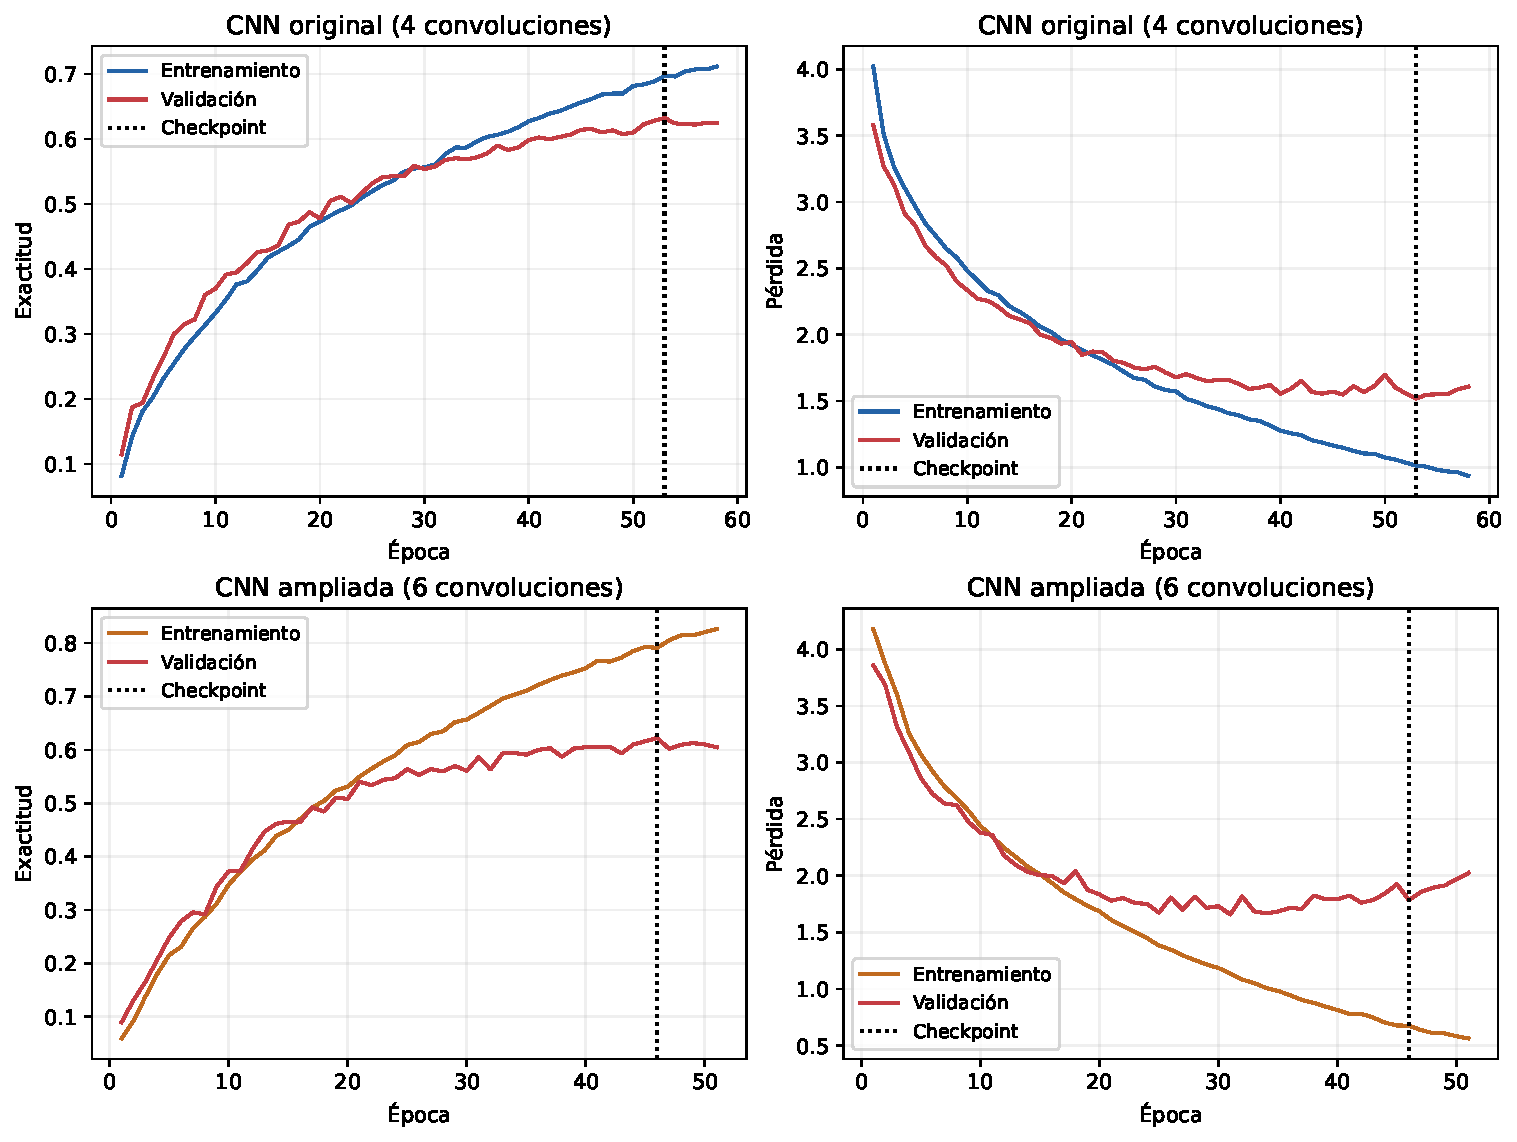
\includegraphics[width=\textwidth,keepaspectratio]{avance4_2026-10-21/figures/comparacion_original_ampliada.pdf}
\caption{CNN original y CNN ampliada: curvas reales por época. El entrenamiento usa aumentos y dropout; la
validación no. Las líneas verticales marcan el mejor checkpoint por F1 macro.}
\label{fig:curvas-av4}
\end{figure*}

\begin{figure*}[p]
\centering
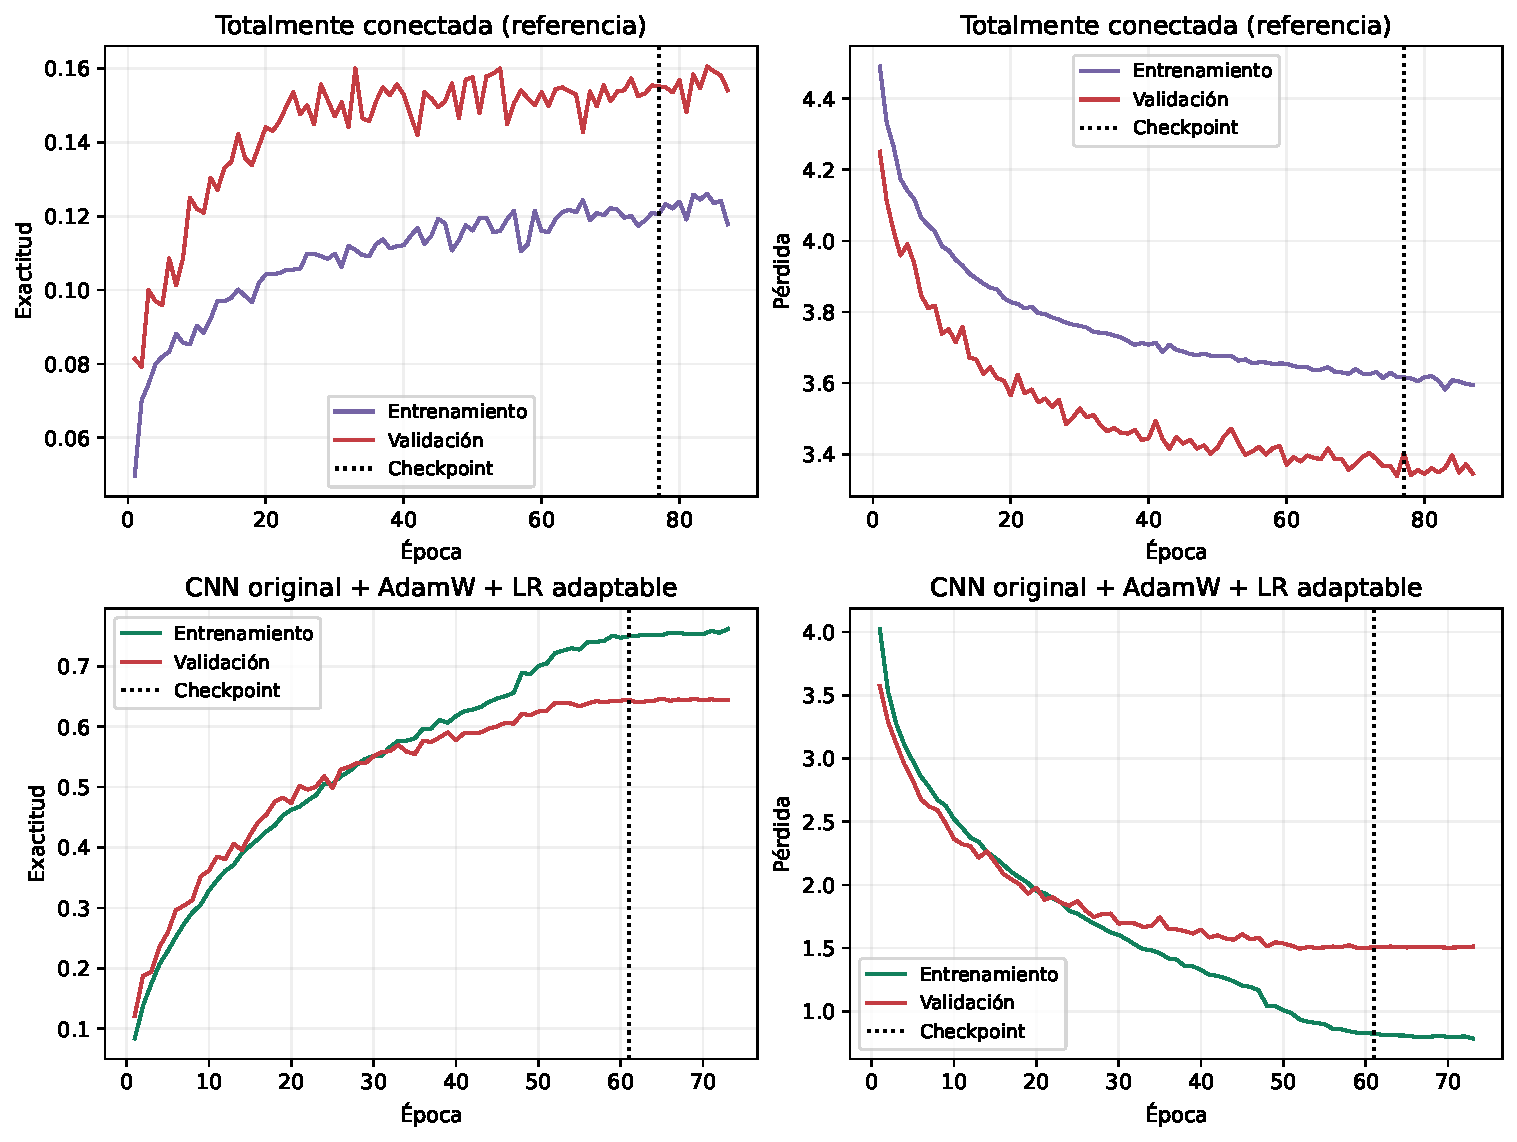
\includegraphics[width=\textwidth,keepaspectratio]{avance4_2026-10-21/figures/comparacion_referencia_regularizada.pdf}
\caption{Curvas de la referencia totalmente conectada y la CNN con la intervención
combinada de regularización. Se mantienen separados sus checkpoints y métricas.}
\label{fig:curvas-ref-reg-av4}
\end{figure*}

\subsection{Técnicas aplicadas y efecto medido}

Todos los modelos usan dropout de 0.5 antes de la salida, aumentos de datos
solo en entrenamiento y parada temprana con restauración del mejor checkpoint.
No se entrenó una ablación sin dropout ni sin aumentos; por eso no se atribuye
por separado una mejora numérica a estas dos técnicas.

La intervención adicional conserva la CNN de cuatro convoluciones, pero utiliza
AdamW con decaimiento de pesos de 0.01 sobre matrices de pesos, excluyendo sesgos.
Se trata de decaimiento desacoplado y no de añadir un término L2 a la pérdida
mostrada. Además, reduce la tasa de aprendizaje a la mitad cuando la pérdida de
validación no mejora durante dos evaluaciones, hasta un mínimo de $10^{-5}$.
La paciencia de parada temprana pasa de 5 a 12 evaluaciones para permitir actuar
a esa reducción. Esta es una intervención combinada: no permite aislar cuánto
aportó el decaimiento, el ajuste de tasa o la paciencia.

Frente a la CNN original, la variante regularizada cambia la exactitud de 63.25\% a 64.44\% (+1.19 puntos porcentuales) y F1 macro de 0.5740 a 0.5745 (+0.0005). Ambos valores se obtienen de los respectivos checkpoints seleccionados por F1 macro sobre la misma validación.

La diferencia de F1 macro es pequeña. Con una sola semilla no se considera evidencia de una mejora robusta o estadísticamente significativa.

Una mejora de exactitud acompañada de una caída de F1 macro no se interpreta como mejora general: el criterio prioritario es el desempeño equilibrado entre las 104 clases. Tampoco se afirma que el sobreajuste desaparezca; se compara la evidencia de las curvas y se conserva el checkpoint que generaliza mejor según la validación disponible.

\begin{figure*}[htbp]
\centering
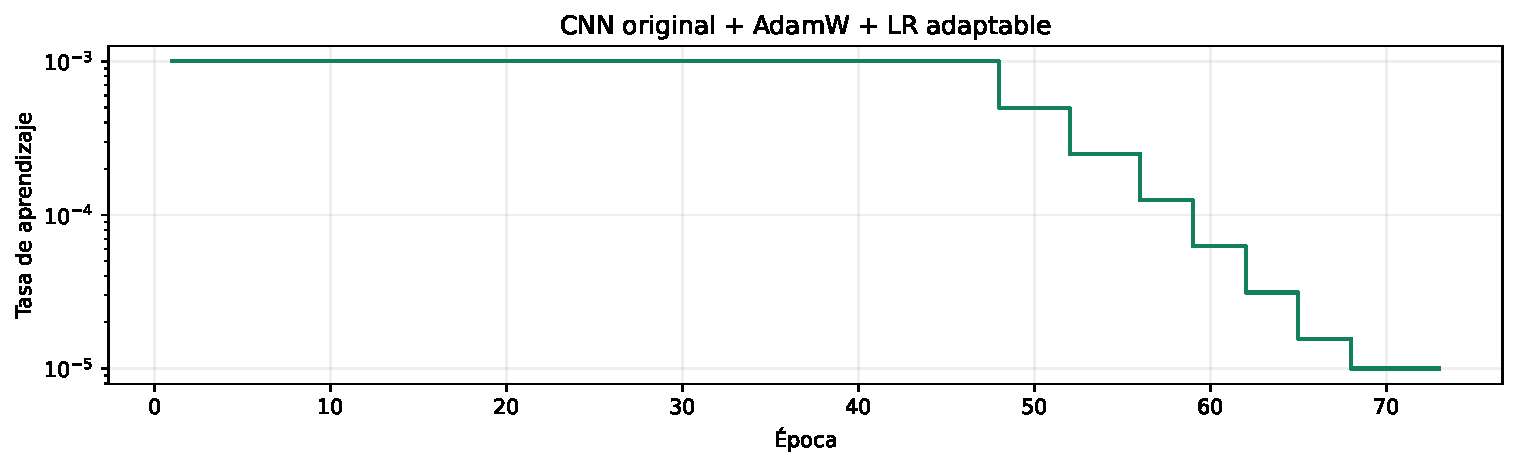
\includegraphics[width=\textwidth]{avance4_2026-10-21/figures/cnn_regularizada/tasa_aprendizaje.pdf}
\caption{Tasa de aprendizaje realmente utilizada en cada época de la variante regularizada. Las reducciones responden al estancamiento de la pérdida de validación.}
\label{fig:lr-av4}
\end{figure*}

\section{Resultados y evaluación}

\subsection{Comparación de modelos}

La Tabla~\ref{tab:resultados-av4} contiene exclusivamente las nuevas ejecuciones
de este avance. Todos los resultados se calcularon sobre 3,712 imágenes reales
de validación, sin aumentos, y corresponden a un checkpoint identificado. Se
conservan los históricos de entrenamiento y las predicciones por imagen.

\begin{table*}[htbp]
\centering
\caption{Resultados nuevos; el checkpoint de cada modelo se selecciona por F1 macro.}
\label{tab:resultados-av4}
\small
\begin{tabular}{lrrrrrr}
\toprule
Modelo & Parámetros & Época & Exactitud (\%) & F1 macro & Pérdida & Tiempo (s) \\
\midrule
MLP de referencia & 9,660,776 & 77 & 15.52 & 0.0280 & 3.403 & 336.7 \\
CNN original & 480,936 & 53 & 63.25 & 0.5740 & 1.520 & 525.8 \\
CNN + 2 convoluciones & 1,218,600 & 46 & 62.23 & 0.5502 & 1.786 & 500.6 \\
CNN + AdamW + LR & 480,936 & 61 & 64.44 & 0.5745 & 1.507 & 605.6 \\
\bottomrule
\end{tabular}
\par\smallskip
\parbox{0.95\textwidth}{\footnotesize Época: checkpoint seleccionado, no número total
de épocas ejecutadas. Tiempo: entrenamiento, excluyendo evaluación y generación
de figuras. La MLP es una referencia reconstruida; no un resultado histórico
atribuible al Avance 3. Una sola semilla por modelo.}
\end{table*}

\begin{figure*}[htbp]
\centering
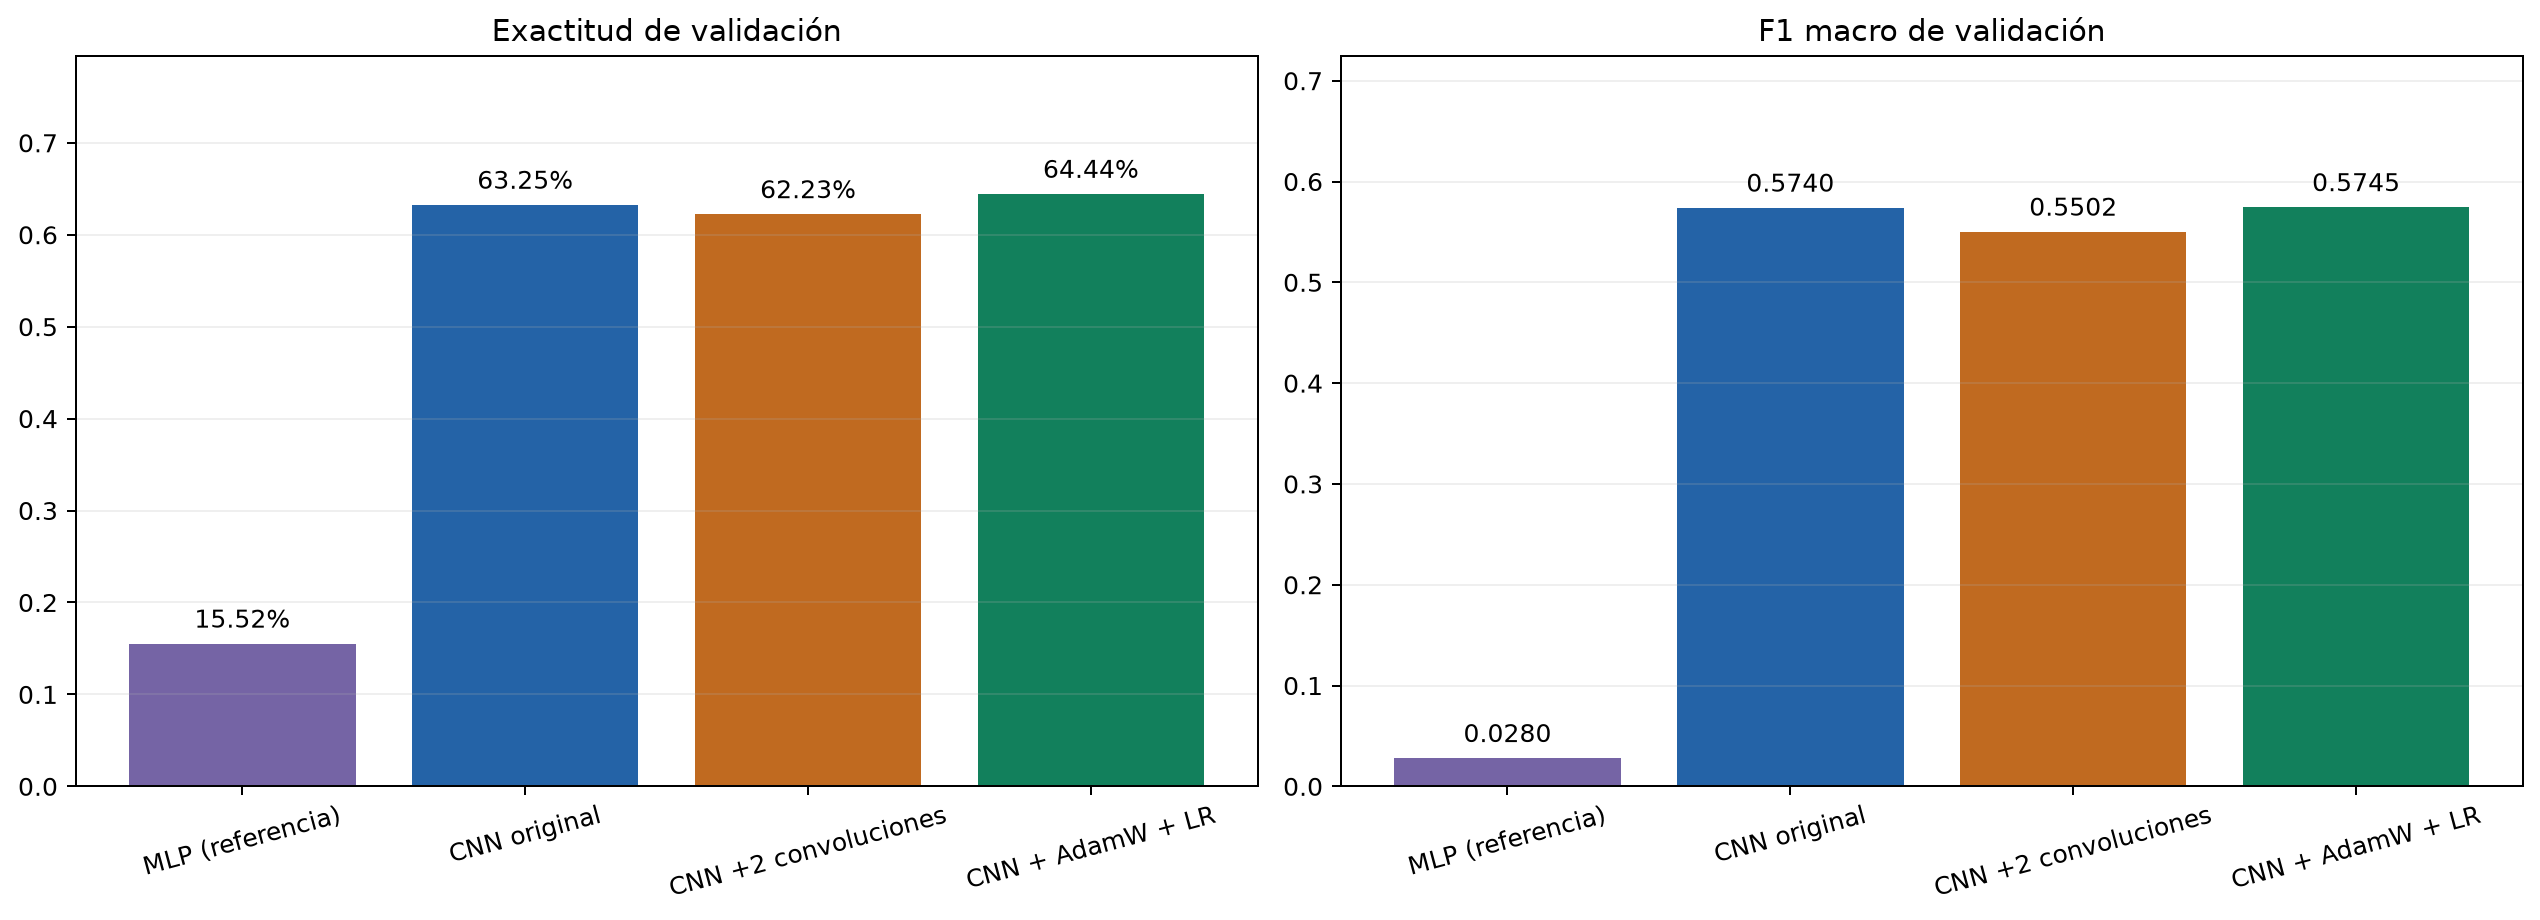
\includegraphics[width=\textwidth]{avance4_2026-10-21/figures/comparacion_metricas.png}
\caption{Exactitud y F1 macro sobre la misma validación. El modelo elegido se
determina por F1 macro y puede diferir del que maximiza la exactitud.}
\label{fig:metricas-av4}
\end{figure*}

\subsection{Puente entre la red totalmente conectada y la CNN}

La CNN original obtuvo 63.25\% de exactitud frente a 15.52\% de la red totalmente conectada de referencia (+47.74 puntos porcentuales). F1 macro cambió de 0.0280 a 0.5740. La MLP tiene 9,660,776 parámetros frente a 480,936 de la CNN.

El resultado es compatible con la ventaja de compartir filtros y preservar vecindarios de píxeles: una CNN puede reutilizar patrones locales sin asignar un peso independiente a cada píxel de cada posición. GAP también limita los parámetros de la etapa densa. Esta explicación es una interpretación arquitectónica del resultado, no una prueba causal aislada; ambas redes tienen distinta capacidad y pueden requerir otros hiperparámetros. Si la MLP presenta baja exactitud tanto en entrenamiento como en validación, su limitación es de ajuste u optimización y no se debe diagnosticar como sobreajuste solo porque rinda peor que la CNN.

La comparación solicitada con el modelo exacto entregado en el Avance 3 queda limitada por la ausencia de ese artefacto identificado. El experimento reconstruido permite comparar familias de modelos en condiciones comunes, sin inventar resultados históricos. El primer intento con Adam a $10^{-3}$ predijo una sola clase (5.82\% de exactitud, F1 macro 0.0011); se conserva como diagnóstico. La referencia final utiliza $10^{-4}$ y mayor paciencia. Esta adaptación de optimización se declara para no atribuir exclusivamente a la arquitectura todas las diferencias observadas.

\subsection{Efecto de agregar dos convoluciones}

La versión de seis convoluciones obtuvo 62.23\% de exactitud y F1 macro 0.5502. Frente a la CNN original, la diferencia es -1.02 puntos de exactitud y -0.0238 de F1 macro. Los parámetros aumentan de 480,936 a 1,218,600. Agregar profundidad incrementa la capacidad de representación, pero no garantiza mejorar validación: también modifica la optimización y puede facilitar el sobreajuste. La conclusión corresponde a esta configuración y semilla, sin afirmar superioridad universal de una profundidad.

\subsection{Modelo elegido y análisis de errores}

Se conserva \textbf{CNN + AdamW + LR}, por tener el mayor F1 macro de esta comparación: 0.5745, con exactitud 64.44\%, pérdida 1.507 y checkpoint en la época 61. La Figura~\ref{fig:confusion-av4} muestra la matriz de confusión normalizada por clase real. La diagonal representa recall por clase; los valores fuera de ella son errores. Se entregan además la matriz de conteos, los CSV de ambas matrices y las predicciones individuales.

\begin{figure*}[p]
\centering
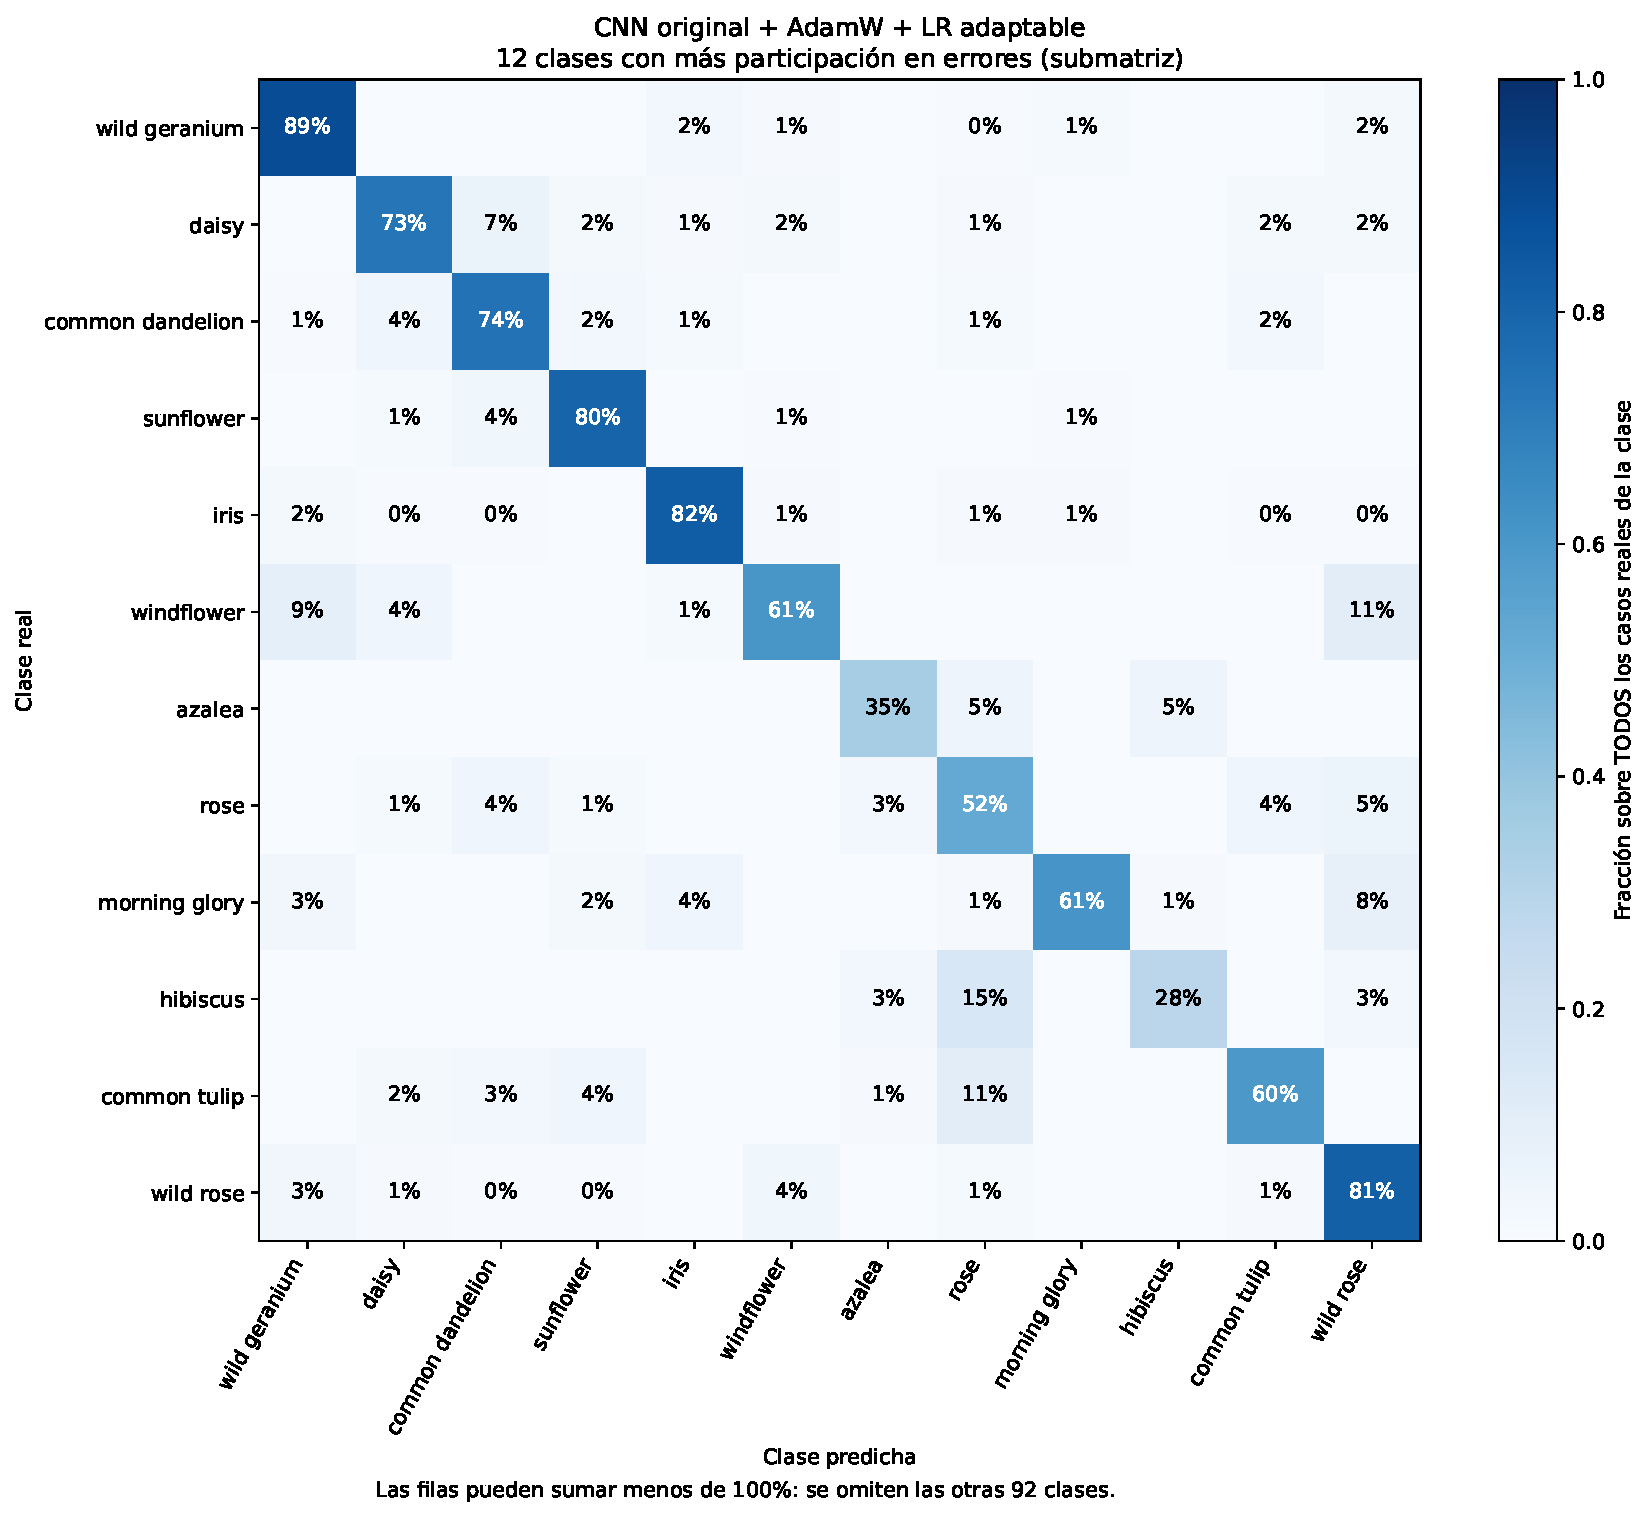
\includegraphics[width=\textwidth]{avance4_2026-10-21/figures/cnn_regularizada/confusiones_principales.pdf}
\caption{Vista legible de las 12 clases con mayor participación en errores. Es una submatriz de la matriz completa: los porcentajes se calculan sobre todos los ejemplos reales de cada clase y las filas mostradas pueden sumar menos de 100\%.}
\label{fig:confusiones-foco-av4}
\end{figure*}

\begin{figure*}[p]
\centering
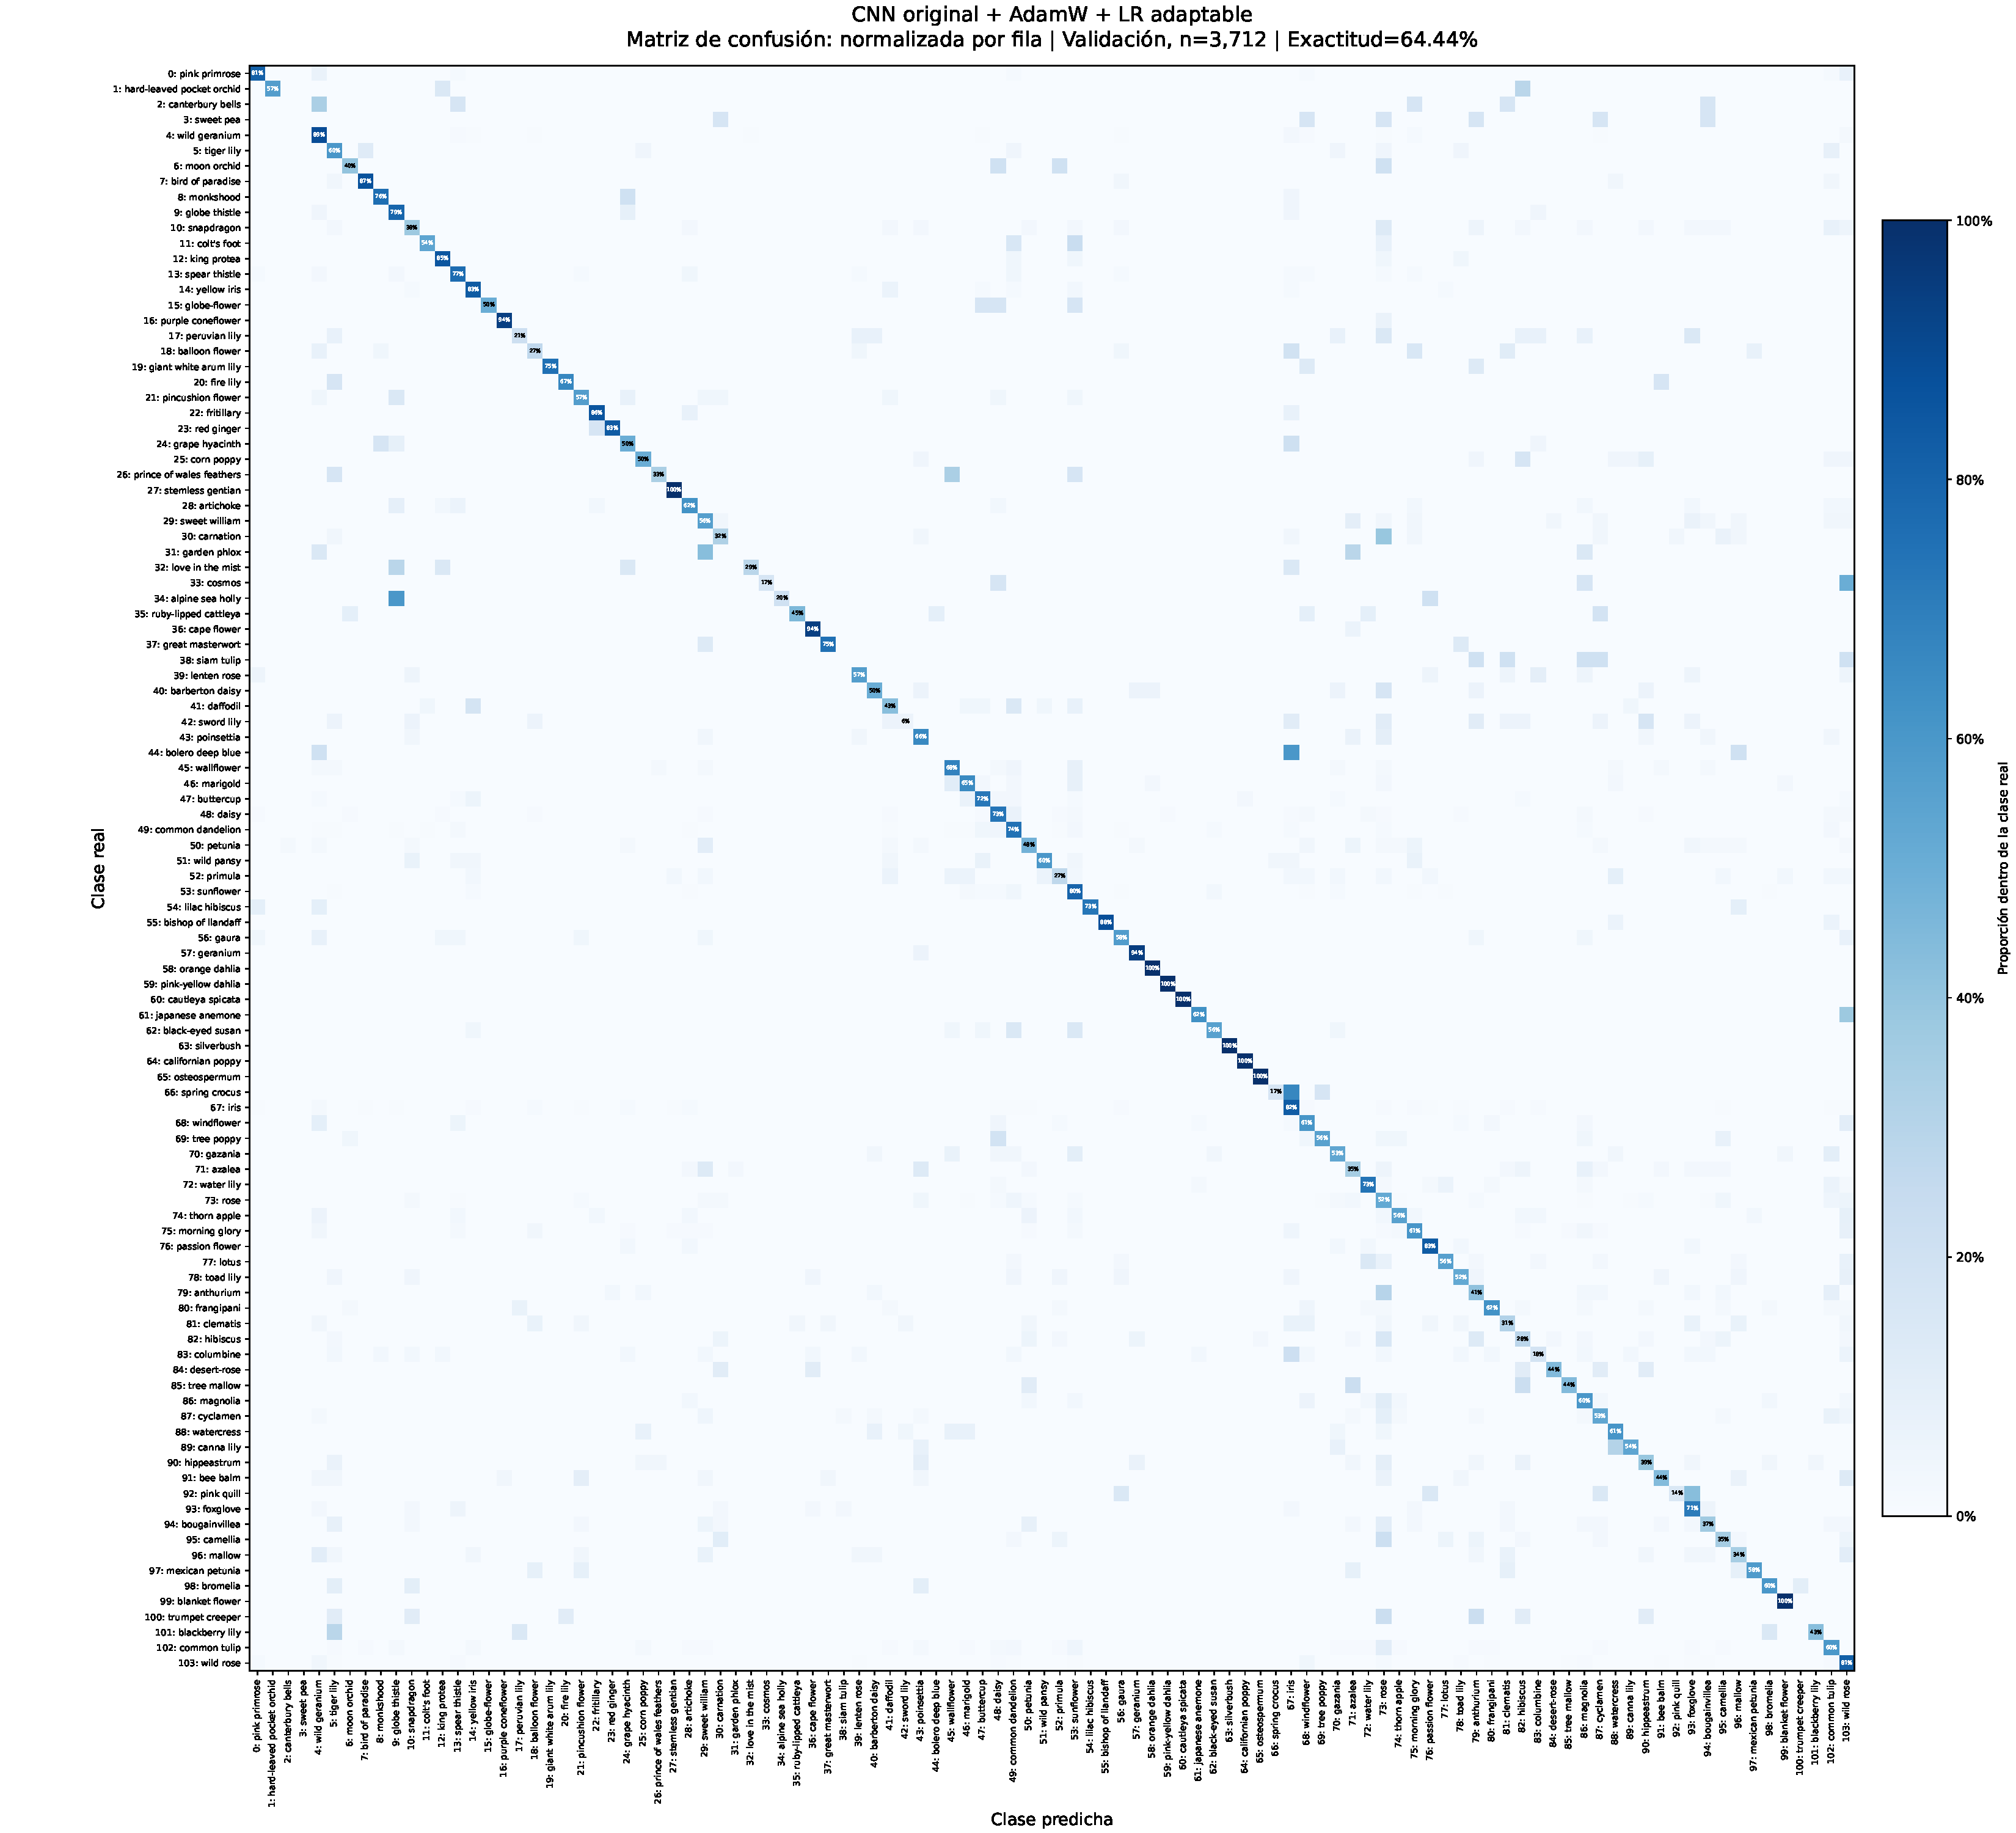
\includegraphics[width=\textwidth,height=0.85\textheight,keepaspectratio]{avance4_2026-10-21/figures/cnn_regularizada/confusion_matrix_normalized.pdf}
\caption{Matriz de confusión del modelo elegido sobre validación. Filas: clase real; columnas: clase predicha. Normalización por fila. Se conserva la versión de alta resolución con las 104 clases.}
\label{fig:confusion-av4}
\end{figure*}

Algunos de los pares más confundidos son:
\begin{itemize}
\item common tulip predicha como rose: 12 imágenes.
\item carnation predicha como rose: 12 imágenes.
\item anthurium predicha como rose: 10 imágenes.
\item windflower predicha como wild rose: 8 imágenes.
\item wild rose predicha como windflower: 8 imágenes.
\end{itemize}
La Figura~\ref{fig:predicciones-av4} ilustra aciertos y errores del checkpoint elegido. Se muestran seis de cada tipo, seleccionados con semilla fija, por lo que esa figura no estima la tasa de error global.

\begin{figure*}[p]
\centering
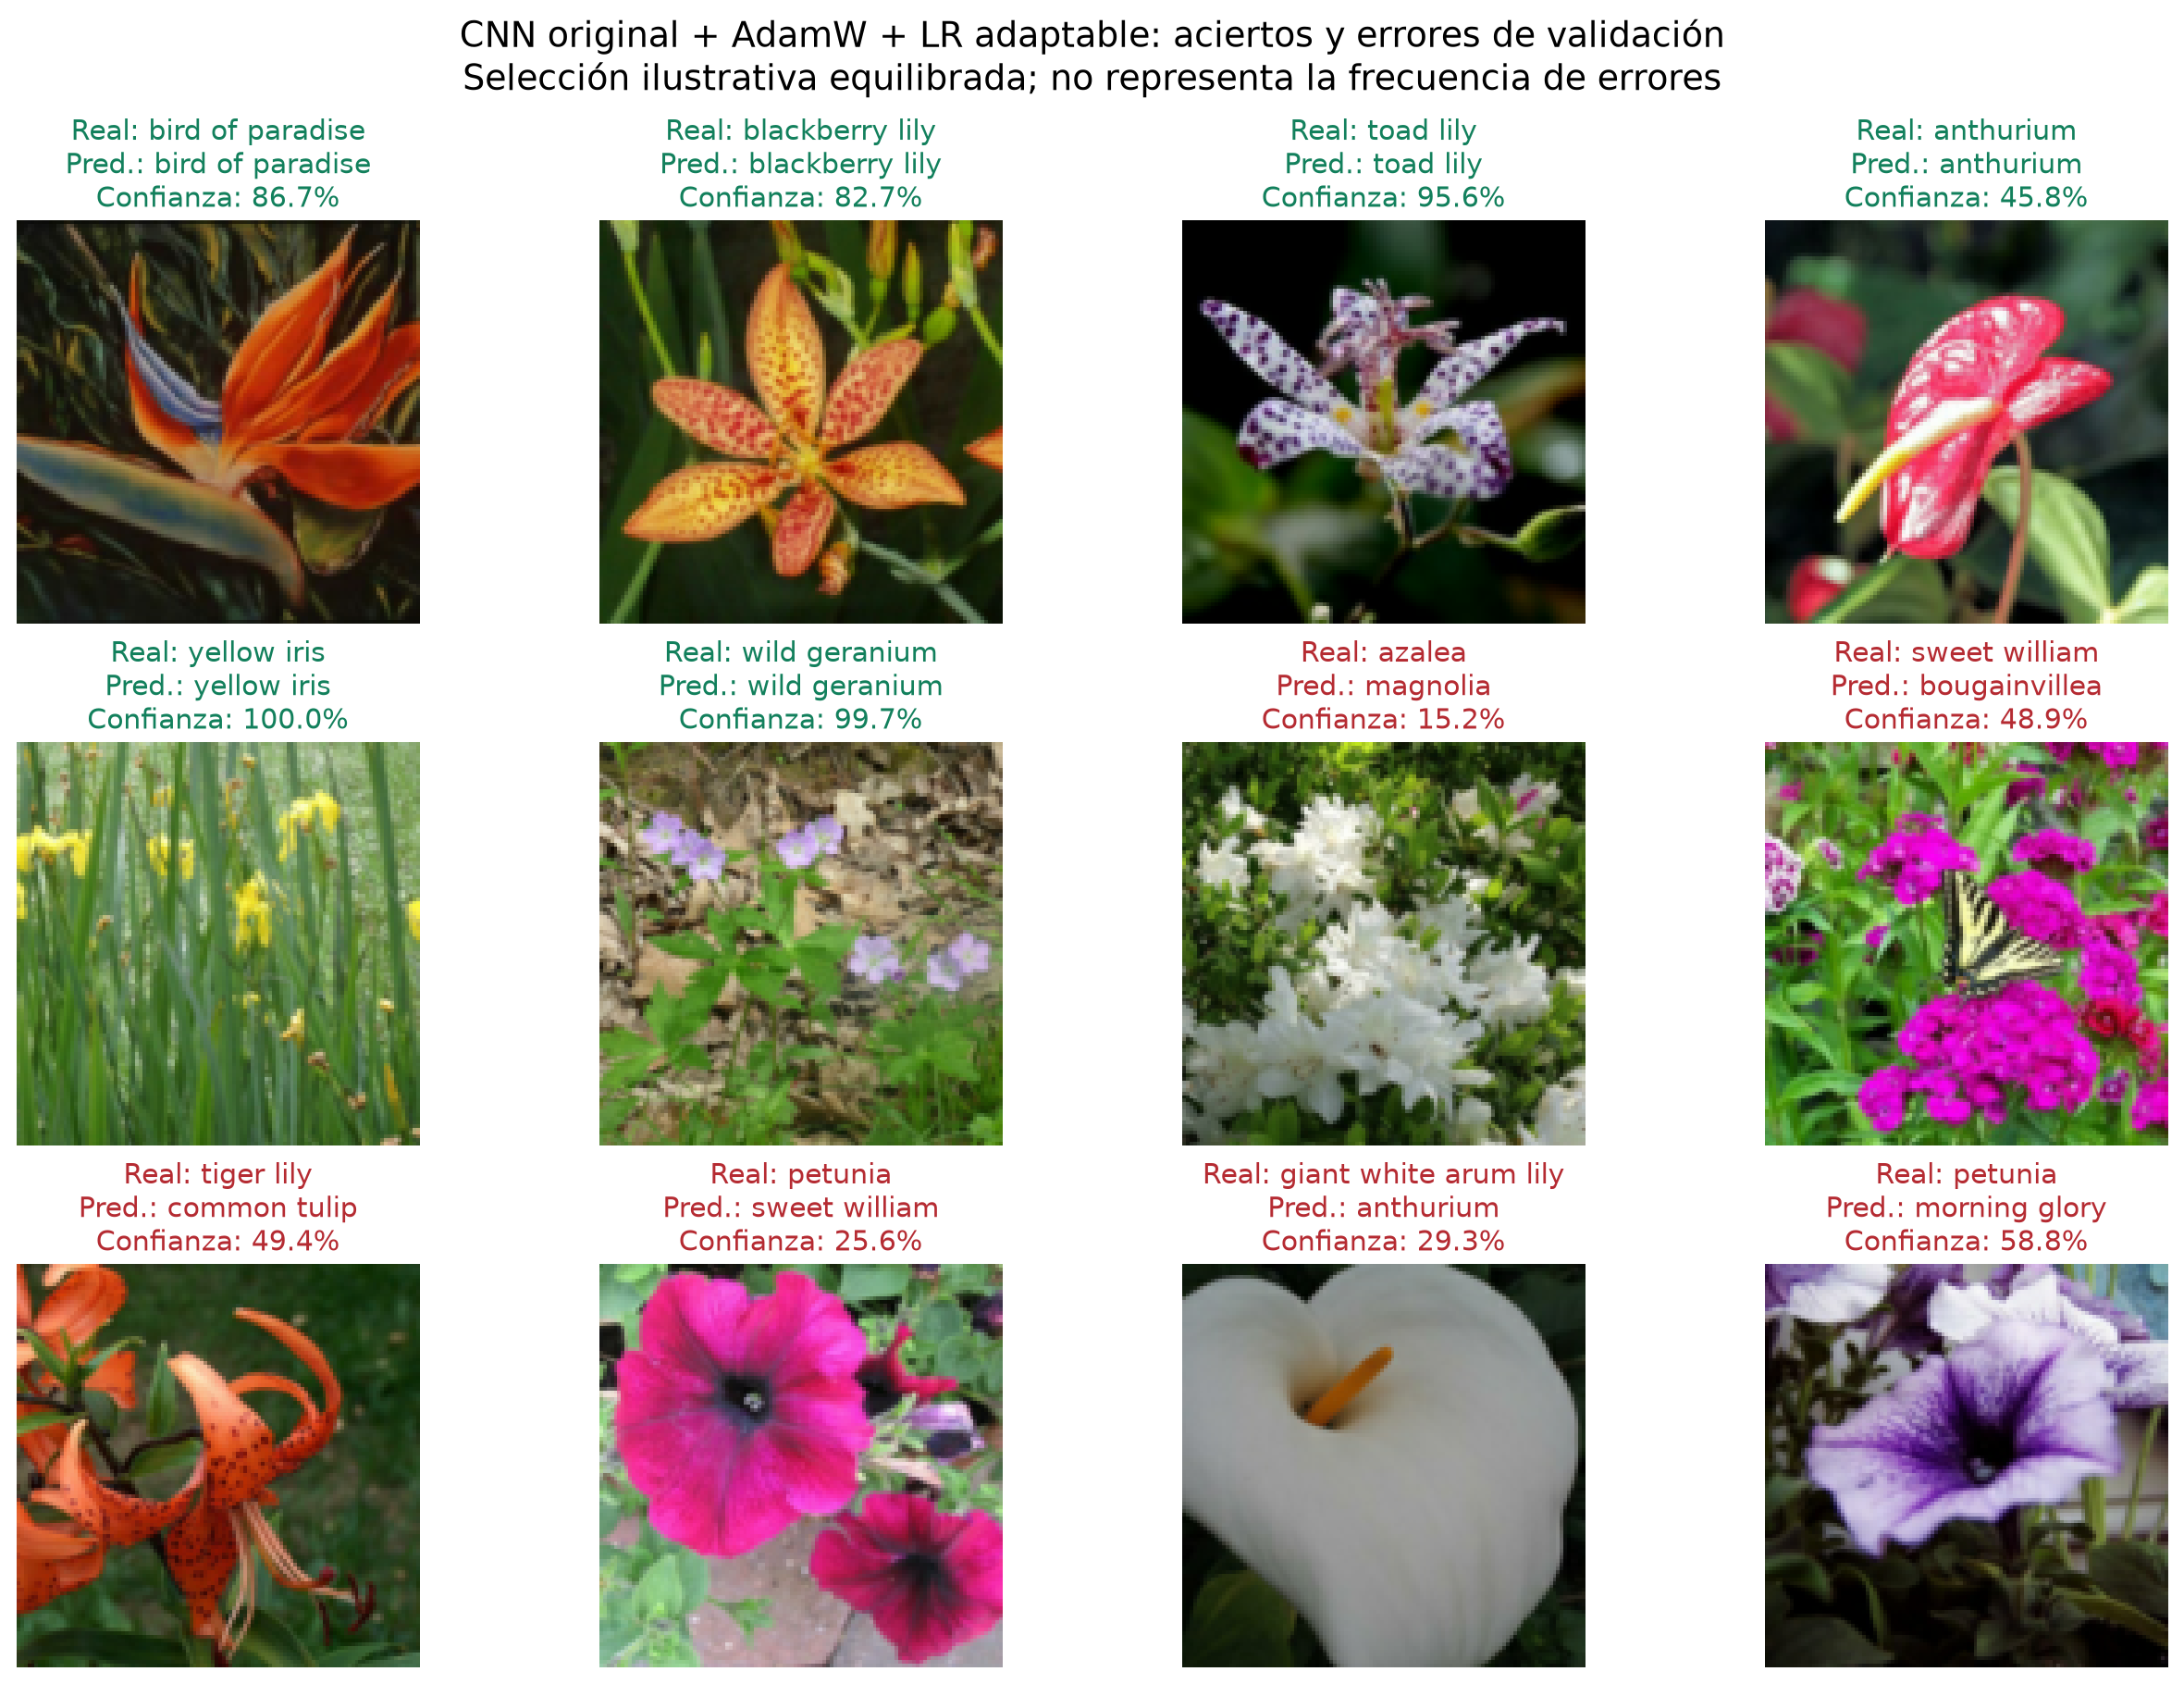
\includegraphics[width=\textwidth]{avance4_2026-10-21/figures/cnn_regularizada/predicciones_ejemplo.png}
\caption{Ejemplos reales de validación con etiqueta verdadera, predicción y confianza softmax. El conjunto mostrado equilibra aciertos y errores solo para facilitar la inspección visual.}
\label{fig:predicciones-av4}
\end{figure*}

\subsection{Conclusiones y limitaciones}

La comparación documenta el cambio de una referencia totalmente conectada a un extractor convolucional, el efecto de aumentar dos convoluciones y el efecto observado de una intervención combinada de regularización. La elección se basa en F1 macro para evitar que las clases numerosas dominen la decisión. Las curvas permiten diagnosticar el comportamiento durante el entrenamiento y justifican conservar checkpoints anteriores al final cuando la validación deja de mejorar.

La validación se utiliza también para selección, los resultados son de una semilla y no se dispone de etiquetas de prueba locales. Harían falta varias semillas, ablaciones controladas y una evaluación independiente para cuantificar incertidumbre y separar el efecto de cada técnica.


\clearpage

\bibliography{references}
\clearpage
\onecolumn
\section*{Anexo: métricas completas y matriz de confusión}
Las métricas se derivan de las 3,712 predicciones de validación del modelo
A4-CNN-AdamW/LR, checkpoint 61. El soporte total es 3,712; los ceros por
clase se conservan al promediar F1 macro. No se trata de métricas de test.
\small
\begin{longtable}{rlrrrr}
\caption{Métricas de las 104 clases. A4-CNN-AdamW/LR, checkpoint 61.}\label{tab:clases-completas}\\
\toprule ID & Clase & Precisión & Recall & F1 & Soporte \\ \midrule
\endfirsthead
\multicolumn{6}{c}{Tabla de clases (continuación)}\\
\toprule ID & Clase & Precisión & Recall & F1 & Soporte \\ \midrule
\endhead
\bottomrule
\endfoot
0 & pink primrose & 0.8767 & 0.8101 & 0.8421 & 79 \\
1 & hard-leaved pocket orchid & 1.0000 & 0.5714 & 0.7273 & 7 \\
2 & canterbury bells & 0.0000 & 0.0000 & 0.0000 & 6 \\
3 & sweet pea & 0.0000 & 0.0000 & 0.0000 & 6 \\
4 & wild geranium & 0.7778 & 0.8878 & 0.8292 & 205 \\
5 & tiger lily & 0.3659 & 0.6000 & 0.4545 & 25 \\
6 & moon orchid & 0.3333 & 0.4000 & 0.3636 & 5 \\
7 & bird of paradise & 0.8438 & 0.8710 & 0.8571 & 31 \\
8 & monkshood & 0.7600 & 0.7600 & 0.7600 & 25 \\
9 & globe thistle & 0.4872 & 0.7917 & 0.6032 & 24 \\
10 & snapdragon & 0.4839 & 0.3750 & 0.4225 & 40 \\
11 & colt's foot & 0.7778 & 0.5385 & 0.6364 & 13 \\
12 & king protea & 0.7931 & 0.8519 & 0.8214 & 27 \\
13 & spear thistle & 0.7108 & 0.7662 & 0.7375 & 77 \\
14 & yellow iris & 0.7333 & 0.8333 & 0.7801 & 66 \\
15 & globe-flower & 1.0000 & 0.5000 & 0.6667 & 6 \\
16 & purple coneflower & 0.9375 & 0.9375 & 0.9375 & 16 \\
17 & peruvian lily & 0.4286 & 0.2143 & 0.2857 & 14 \\
18 & balloon flower & 0.3684 & 0.2692 & 0.3111 & 26 \\
19 & giant white arum lily & 1.0000 & 0.7500 & 0.8571 & 8 \\
20 & fire lily & 0.8000 & 0.6667 & 0.7273 & 6 \\
21 & pincushion flower & 0.5714 & 0.5714 & 0.5714 & 28 \\
22 & fritillary & 0.8000 & 0.8571 & 0.8276 & 14 \\
23 & red ginger & 0.8333 & 0.8333 & 0.8333 & 6 \\
24 & grape hyacinth & 0.4138 & 0.5000 & 0.4528 & 24 \\
25 & corn poppy & 0.6316 & 0.5000 & 0.5581 & 24 \\
26 & prince of wales feathers & 0.5000 & 0.3333 & 0.4000 & 6 \\
27 & stemless gentian & 0.7692 & 1.0000 & 0.8696 & 10 \\
28 & artichoke & 0.5676 & 0.6176 & 0.5915 & 34 \\
29 & sweet william & 0.3462 & 0.5625 & 0.4286 & 32 \\
30 & carnation & 0.4000 & 0.3226 & 0.3571 & 31 \\
31 & garden phlox & 0.0000 & 0.0000 & 0.0000 & 7 \\
32 & love in the mist & 0.6667 & 0.2857 & 0.4000 & 7 \\
33 & cosmos & 1.0000 & 0.1667 & 0.2857 & 6 \\
34 & alpine sea holly & 1.0000 & 0.2000 & 0.3333 & 5 \\
35 & ruby-lipped cattleya & 0.8333 & 0.4545 & 0.5882 & 11 \\
36 & cape flower & 0.8000 & 0.9412 & 0.8649 & 17 \\
37 & great masterwort & 0.7500 & 0.7500 & 0.7500 & 8 \\
38 & siam tulip & 0.0000 & 0.0000 & 0.0000 & 5 \\
39 & lenten rose & 0.6316 & 0.5714 & 0.6000 & 21 \\
40 & barberton daisy & 0.5625 & 0.5000 & 0.5294 & 18 \\
41 & daffodil & 0.4444 & 0.4286 & 0.4364 & 28 \\
42 & sword lily & 0.3333 & 0.0556 & 0.0952 & 18 \\
43 & poinsettia & 0.4565 & 0.6562 & 0.5385 & 32 \\
44 & bolero deep blue & 0.0000 & 0.0000 & 0.0000 & 5 \\
45 & wallflower & 0.7083 & 0.6800 & 0.6939 & 50 \\
46 & marigold & 0.6000 & 0.6486 & 0.6234 & 37 \\
47 & buttercup & 0.7639 & 0.7237 & 0.7432 & 76 \\
48 & daisy & 0.7258 & 0.7317 & 0.7287 & 123 \\
49 & common dandelion & 0.7052 & 0.7439 & 0.7240 & 164 \\
50 & petunia & 0.6364 & 0.4828 & 0.5490 & 58 \\
51 & wild pansy & 0.8571 & 0.6000 & 0.7059 & 30 \\
52 & primula & 0.4737 & 0.2727 & 0.3462 & 33 \\
53 & sunflower & 0.6948 & 0.7985 & 0.7431 & 134 \\
54 & lilac hibiscus & 1.0000 & 0.7273 & 0.8421 & 11 \\
55 & bishop of llandaff & 1.0000 & 0.8824 & 0.9375 & 17 \\
56 & gaura & 0.5556 & 0.5769 & 0.5660 & 26 \\
57 & geranium & 0.7391 & 0.9444 & 0.8293 & 18 \\
58 & orange dahlia & 0.8333 & 1.0000 & 0.9091 & 10 \\
59 & pink-yellow dahlia & 0.9444 & 1.0000 & 0.9714 & 17 \\
60 & cautleya spicata & 1.0000 & 1.0000 & 1.0000 & 8 \\
61 & japanese anemone & 0.6250 & 0.6250 & 0.6250 & 8 \\
62 & black-eyed susan & 0.6818 & 0.5556 & 0.6122 & 27 \\
63 & silverbush & 1.0000 & 1.0000 & 1.0000 & 8 \\
64 & californian poppy & 0.8889 & 1.0000 & 0.9412 & 16 \\
65 & osteospermum & 0.9000 & 1.0000 & 0.9474 & 9 \\
66 & spring crocus & 0.5000 & 0.1667 & 0.2500 & 6 \\
67 & iris & 0.7833 & 0.8246 & 0.8034 & 228 \\
68 & windflower & 0.5974 & 0.6053 & 0.6013 & 76 \\
69 & tree poppy & 0.8824 & 0.5556 & 0.6818 & 27 \\
70 & gazania & 0.5000 & 0.5333 & 0.5161 & 30 \\
71 & azalea & 0.3784 & 0.3500 & 0.3636 & 40 \\
72 & water lily & 0.7347 & 0.7347 & 0.7347 & 49 \\
73 & rose & 0.3763 & 0.5224 & 0.4375 & 134 \\
74 & thorn apple & 0.7143 & 0.5556 & 0.6250 & 36 \\
75 & morning glory & 0.7013 & 0.6067 & 0.6506 & 89 \\
76 & passion flower & 0.8056 & 0.8286 & 0.8169 & 35 \\
77 & lotus & 0.7667 & 0.5610 & 0.6479 & 41 \\
78 & toad lily & 0.5200 & 0.5200 & 0.5200 & 25 \\
79 & anthurium & 0.3415 & 0.4118 & 0.3733 & 34 \\
80 & frangipani & 0.8235 & 0.6222 & 0.7089 & 45 \\
81 & clematis & 0.3750 & 0.3103 & 0.3396 & 29 \\
82 & hibiscus & 0.3333 & 0.2821 & 0.3056 & 39 \\
83 & columbine & 0.4000 & 0.1818 & 0.2500 & 33 \\
84 & desert-rose & 0.6667 & 0.4444 & 0.5333 & 9 \\
85 & tree mallow & 0.6667 & 0.4444 & 0.5333 & 9 \\
86 & magnolia & 0.4038 & 0.6000 & 0.4828 & 35 \\
87 & cyclamen & 0.5476 & 0.5349 & 0.5412 & 43 \\
88 & watercress & 0.5667 & 0.6071 & 0.5862 & 28 \\
89 & canna lily & 0.6364 & 0.5385 & 0.5833 & 13 \\
90 & hippeastrum & 0.4286 & 0.3871 & 0.4068 & 31 \\
91 & bee balm & 0.7000 & 0.4375 & 0.5385 & 32 \\
92 & pink quill & 0.5000 & 0.1429 & 0.2222 & 7 \\
93 & foxglove & 0.5472 & 0.7073 & 0.6170 & 41 \\
94 & bougainvillea & 0.4828 & 0.3684 & 0.4179 & 38 \\
95 & camellia & 0.3939 & 0.3514 & 0.3714 & 37 \\
96 & mallow & 0.4348 & 0.3448 & 0.3846 & 29 \\
97 & mexican petunia & 0.7000 & 0.5833 & 0.6364 & 12 \\
98 & bromelia & 0.5455 & 0.6000 & 0.5714 & 10 \\
99 & blanket flower & 0.7000 & 1.0000 & 0.8235 & 7 \\
100 & trumpet creeper & 0.0000 & 0.0000 & 0.0000 & 9 \\
101 & blackberry lily & 0.7500 & 0.4286 & 0.5455 & 7 \\
102 & common tulip & 0.6182 & 0.5965 & 0.6071 & 114 \\
103 & wild rose & 0.6875 & 0.8148 & 0.7458 & 216 \\
\end{longtable}

\clearpage
\begin{figure}[p]
\centering
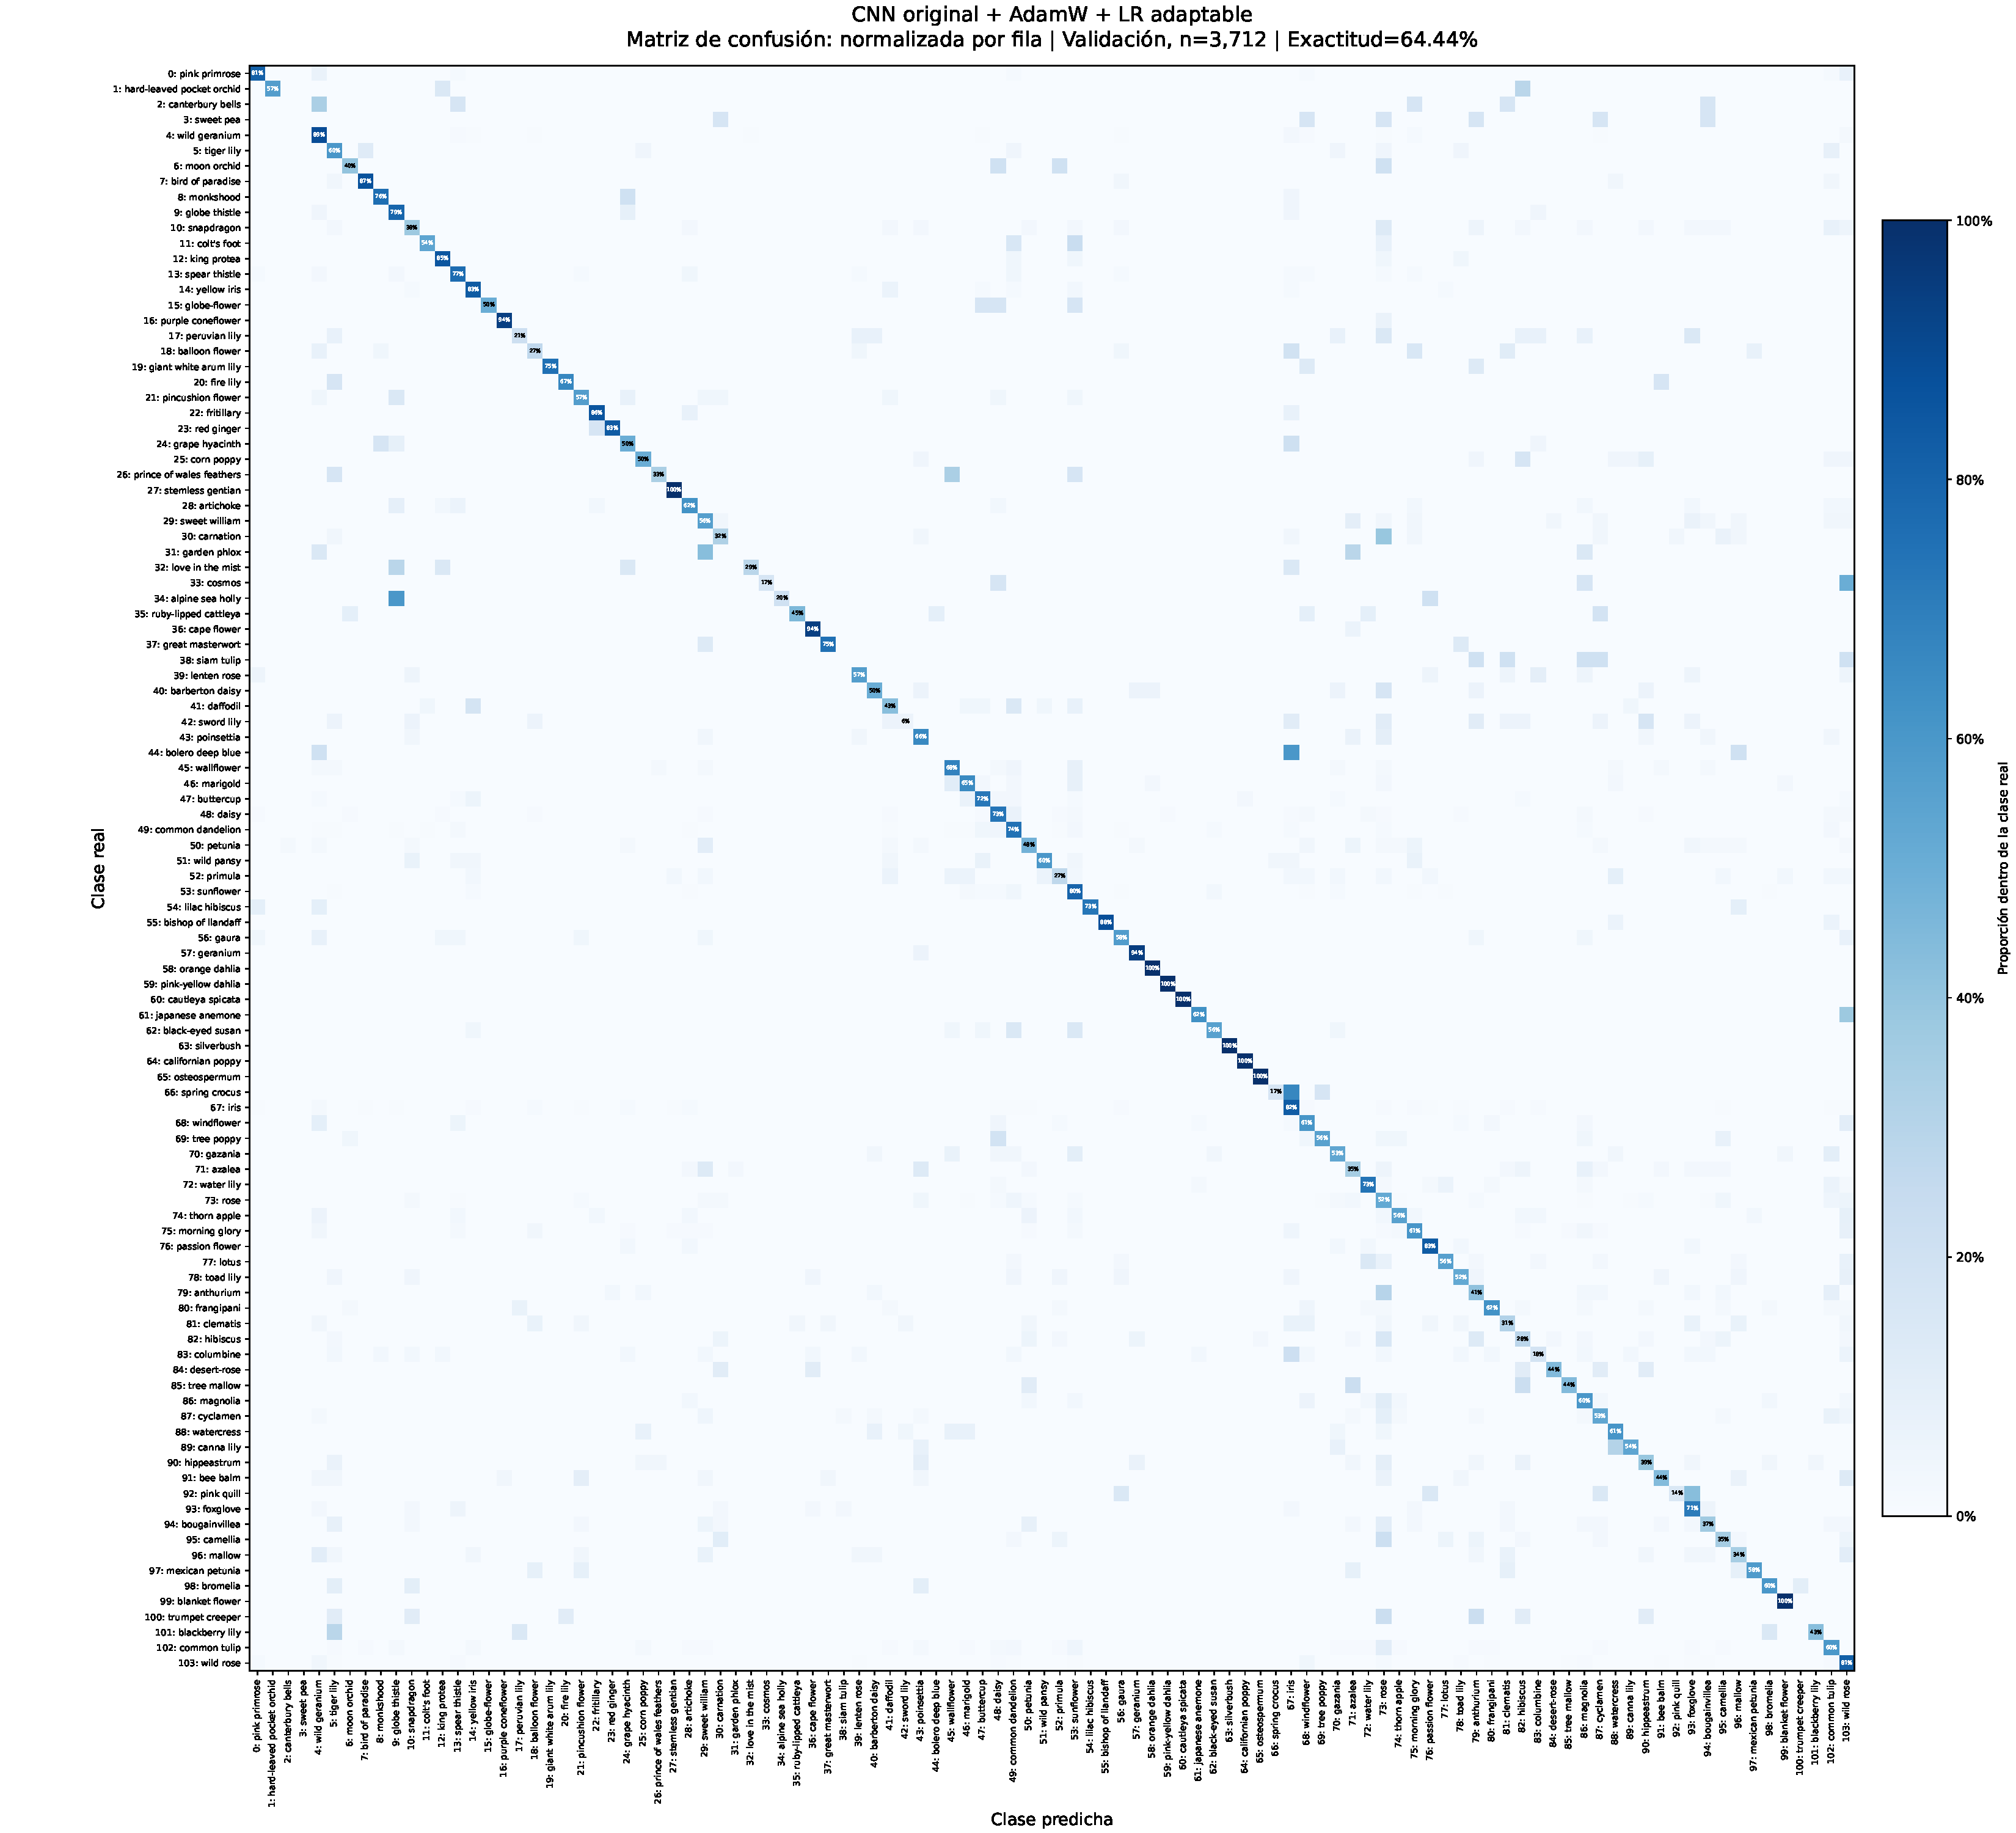
\includegraphics[width=\textwidth,height=0.85\textheight,keepaspectratio]{avance4_2026-10-21/figures/cnn_regularizada/confusion_matrix_normalized.pdf}
\caption{Matriz completa normalizada por clase real del modelo seleccionado
(104 clases). La diagonal representa recall; la vista de foco del cuerpo permite
leer los errores más frecuentes.}\label{fig:matriz-completa}
\end{figure}

\end{document}
